%# -*- coding: utf-8 -*-
\documentclass[a4paper]{article}
\usepackage{graphicx}
\usepackage{epstopdf}
\usepackage{pstool}
\usepackage{titlesec, titletoc}     %设置标题格式
%\usepackage{CJKnumb}               %中文数字
\usepackage[unicode=true,
            CJKbookmarks=true,
            colorlinks=true,
            linkcolor=black]{hyperref}
\usepackage[nocap,nopunct,space]{ctex}
\usepackage{wrapfig}
\usepackage{fancyhdr}   %页眉页脚
\usepackage{ifthen}
\usepackage{longtable}
\usepackage{listings}               %代码排版
\usepackage{color}                  %代码排版背景颜色
\usepackage[labelfont=bf,up,
            textfont=it,up]{caption}
\usepackage{subcaption}
\usepackage{amsmath}
\usepackage{makecell}
\usepackage[americanvoltages,americancurrents,americanresistors,%
    americaninductors,americanports,siunitx,emptydiodes,%
  arrowmos,nopmosdot]{circuitikz}
\usepackage{tikz}
\usepackage{siunitx}
\usepackage{multirow}

\definecolor{gray}{rgb}{0.9,0.9,0.9}
\definecolor{shadecolor}{gray}{0.85}

%\usepackage[autolinebreaks]{mcode}
\lstset{aboveskip=.8em,
xleftmargin=1em,
xrightmargin=1em,
language={},
basicstyle=\footnotesize\ttfamily,
backgroundcolor=\color{gray},
}

%设置各字体
\setCJKmainfont[BoldFont={FZDaHei-B02S},
    ItalicFont={Adobe Kaiti Std}]{Adobe Song Std}
\setCJKmonofont{Adobe Fangsong Std}
\setmainfont[Mapping=tex-text]{Times New Roman}
\setsansfont{Arial}
\setmonofont{Courier New}

\newcommand{\HUGE}{\fontsize{29pt}{29pt}\selectfont}

%\titleformat{\contents}{\Huge\bfseries}{\vspace{0.3cm}}{1em} {}
%\titleformat{\section}{\centering\fontsize{16pt}{20pt}\selectfont\bfseries}{\vspace{0.3cm}}{1em} {\vspace{.8cm}}
%\titleformat{\subsection}{\fontsize{12pt}{15pt}\selectfont\bfseries}{\arabic{subsection}.}{1em} {}
%\titleformat{\subsubsection}{\large\bfseries}{\arabic{subsection}.\arabic{subsubsection}}{1em} {\vspace{.1em}}

\headheight=13pt

% 本文档自定义变量

\renewcommand{\d}[1]{\ensuremath{\operatorname{d}\!{#1}}}

\newcommand{\lsq}{\ensuremath{\protect{[}}}
\newcommand{\rsq}{\ensuremath{\protect{]}}}

%\renewcommand{\d}{\ensuremath{{d}}}
\newcommand{\uV}{\si{\volt}}
\newcommand{\umV}{\si{\milli\volt}}
\newcommand{\uuV}{\si{\micro\volt}}

\newcommand{\umA}{\si{\milli\ampere}}
\newcommand{\uuA}{\si{\micro\ampere}}

\newcommand{\upF}{\si{\pico\farad}}
\newcommand{\ufF}{\si{\femto\farad}}
\newcommand{\unF}{\si{\nano\farad}}

\newcommand{\upJ}{\si{\pico\joule}}

\newcommand{\unm}{\si{\nano\metre}}
\newcommand{\uum}{\si{\micro\metre}}
\newcommand{\uumsq}{\si{\micro\metre^2}}

\newcommand{\uns}{\si{\nano\second}}
\newcommand{\ups}{\si{\pico\second}}

\newcommand{\uuW}{\si{\micro\watt}}
\newcommand{\umW}{\si{\milli\watt}}

\newcommand{\uO}{\si{\ohm}}
\newcommand{\ukO}{\si{\kilo\ohm}}

\newcommand{\uS}{\si{\siemens}}
\newcommand{\umS}{\si{\milli\siemens}}

\newcommand{\uPV}{\si{\volt^{-1}}}
\newcommand{\uAPV}{\si{\ampere\per\volt}}
\newcommand{\umAPV}{\si{\milli\ampere\per\volt}}

\newcommand{\uHz}{\si{\hertz}}
\newcommand{\uMHz}{\si{\mega\hertz}}
\newcommand{\ukHz}{\si{\kilo\hertz}}

\newcommand{\udB}{\si{\deci\bel}}
\newcommand{\uVVPHz}{\si{\volt^2\per\hertz}}

\newcommand{\udeg}{\si{\degree}}

\newcommand{\ten}[1]{\ensuremath{\times10^{#1}}}

\newcommand{\dM}[1]{\mathrm{M}_\mathrm{#1}}
\newcommand{\DM}[1]{$\dM{#1}$}
\newcommand{\dR}[1]{\mathrm{R}_\mathrm{#1}}
\newcommand{\DR}[1]{$\dR{#1}$}
\newcommand{\dC}[1]{\mathrm{C}_\mathrm{#1}}
\newcommand{\DC}[1]{$\dC{#1}$}


%% circuitikz 
\makeatletter
\ctikzset{lx/.code args={#1 and #2}{ 
  \pgfkeys{/tikz/circuitikz/bipole/label/name=\parbox{1cm}{\centering #1  \\ #2}}
    \ctikzsetvalof{bipole/label/unit}{}
    \ifpgf@circ@siunitx 
        \pgf@circ@handleSI{#2}
        \ifpgf@circ@siunitx@res 
            \edef\pgf@temp{\pgf@circ@handleSI@val}
            \pgfkeyslet{/tikz/circuitikz/bipole/label/name}{\pgf@temp}
            \edef\pgf@temp{\pgf@circ@handleSI@unit}
            \pgfkeyslet{/tikz/circuitikz/bipole/label/unit}{\pgf@temp}
        \else
        \fi
    \else
    \fi
}}

\ctikzset{lx^/.style args={#1 and #2}{ 
    lx=#2 and #1,
    \circuitikzbasekey/bipole/label/position=90 } 
}

\ctikzset{lx_/.style args={#1 and #2}{ 
    lx=#1 and #2,
    \circuitikzbasekey/bipole/label/position=-90 } 
}
\makeatother

%% External resources
\newcommand{\gmidb}{9.53\uPV}
\newcommand{\gmidA}{9.09\uPV}
\newcommand{\gmidB}{17.79\uPV}
\newcommand{\gmidC}{18.24\uPV}
\newcommand{\gmidD}{11.54\uPV}
\newcommand{\gmidE}{11.83\uPV}
\newcommand{\gmidBa}{13.36\uPV}
\newcommand{\gmidCa}{13.69\uPV}
\newcommand{\gmidDa}{10.76\uPV}
\newcommand{\gmidEa}{11.03\uPV}
\newcommand{\gmidFa}{2.08\uPV}
\newcommand{\gmidFb}{8.23\uPV}
\newcommand{\gmidFc}{9.23\uPV}
\newcommand{\gmidGa}{10.21\uPV}
\newcommand{\gmidGb}{8.17\uPV}
\newcommand{\gmidGc}{9.82\uPV}
\newcommand{\gmidGd}{2.52\uPV}
\newcommand{\gmidHa}{10.24\uPV}
\newcommand{\gmidHb}{10.42\uPV}
\newcommand{\gmidHc}{9.05\uPV}
\newcommand{\idb}{0.207\umA}
\newcommand{\idA}{3.451\umA}
\newcommand{\idDa}{1.101\umA}
\newcommand{\idEa}{1.075\umA}
\newcommand{\idFa}{0.225\umA}
\newcommand{\idGa}{0.220\umA}
\newcommand{\idHa}{0.234\umA}

\newcommand{\sizeBa}{302.72/0.533}
\newcommand{\sizeGb}{83.70/0.633}
\newcommand{\sizeGc}{30.27/0.533}
\newcommand{\sizeGd}{6.05/0.533}
\newcommand{\sizeHb}{169.49/0.633}
\newcommand{\sizeHa}{169.49/0.633}
\newcommand{\sizeGa}{161.42/0.633}
\newcommand{\sizeb}{21.96/0.410}
\newcommand{\sizeE}{1614.20/0.855}
\newcommand{\sizeB}{653.87/0.410}
\newcommand{\sizeA}{439.28/0.410}
\newcommand{\sizeD}{1614.20/0.855}
\newcommand{\sizeC}{653.87/0.410}
\newcommand{\sizeCa}{302.72/0.533}
\newcommand{\sizeHc}{21.96/0.410}
\newcommand{\sizeDa}{837.01/0.633}
\newcommand{\sizeFb}{87.89/0.633}
\newcommand{\sizeFa}{17.58/0.633}
\newcommand{\sizeFc}{21.96/0.410}
\newcommand{\sizeEa}{837.01/0.633}

\newcommand{\moslabel}[3]{\shortstack{$\dM{#1}$\\{\scriptsize$#2$}\\{\scriptsize$#3$}}}

\begin{document}

\begin{titlepage}

% 首行的位置往上调整。但vspace前面需要有东西才会起效。
\phantom{Start!}
\vspace{-1.7cm}

\begin{flushleft}

\emph{\Large 清华大学微纳电子系}\\[0.2cm]
\emph{\Large 模拟集成电路分析与设计}\\[4.2cm]     % 课程

% Title
{ \HUGE \bfseries OTA放大器设计}\\[0.4cm]    % 主标题
{ \huge \bfseries 设计报告}             % 副标题

\end{flushleft}

\vfill

\begin{flushright}

{
\newcommand{\pillar}{ {\Huge \phantom{A}} } %一种统一的方法提高行高
\large \begin{tabular}{lll}
  \pillar 姓名 & 孙泽雷 & 2010011210 \\
  \pillar&牟瞳 & 2010011204          \\
  \pillar&吕若辰 & 2010011201        \\
  \pillar 班级 & 微02 &               \\
  \pillar 报告日期 & \multicolumn{2}{l}{2013年6月28日}  \\
\end{tabular}
}

\end{flushright}

\end{titlepage}

\newpage

\pagenumbering{arabic}
\pagestyle{fancy}
\fancyhead{}    % 清空设置
\fancyhead[HL]{清华大学电子工程系}
\fancyhead[HR]{数字逻辑与处理器基础实验}    %课程

% Page 1: Outline of your design, justifications of key design decisions; 
% comparison with alternatives.

\section{综述}

本电路设计了一个低功耗OTA放大器。

采用的基本电路是Telescope单级放大器,它的优点是在具有较大增益的同时,
功耗较低。其缺点是比起折叠Cascode放大器而言摆幅较低,从而导致动态增益
的目标会更难完成,不过由于本次设计目标中动态增益的要求还算适中,
为了达到更低功耗的目的,仍采用Telescope放大电路。设计的过程也表明,
设计时的主要限制因素并非动态增益(而是静态误差和动态时间之间的折衷)。

采用了基于理想压控电流源的共模反馈,共模基准电压为$1.6\uV$。

\newpage

\section{电路结构及参数}

% Page 2: Schematic diagram of final design, with component values and bias 
% currents clearly labeled. Show component values right next to the components, 
% and currents next to the branches (i.e., absolutely, positively do not make us 
% refer to a look-up table). Annotate all transistors with the chosen gm/ID value.
\subsection{Telescopic电路结构}
Telescopic电路图及各项器件的参数如图\ref{circuit}。

图中采用简单镜像电流源对 Telescopic 的支路电流进行偏置。
\begin{figure}[htb!]
  \centering
  \begin{center}
  \scalebox{0.7}{
  \begin{circuitikz}
    \pgfmathsetmacro{\xa}{0}        % B
    \pgfmathsetmacro{\xb}{2.2}        % left bias 1
    \pgfmathsetmacro{\xc}{4.4}      % left bias 2
    \pgfmathsetmacro{\xd}{7.0}      % M1
    \pgfmathsetmacro{\xe}{8.9}      % M0
    \pgfmathsetmacro{\xm}{9.6}      % M6CD
    \pgfmathsetmacro{\xf}{10.6}      % M2

    \pgfmathsetmacro{\xfb}{13.0}      % VOC feedback

    \pgfmathsetmacro{\ya}{0  }
    \pgfmathsetmacro{\yb}{4  }      % M1,2
    \pgfmathsetmacro{\yc}{4.5}
    \pgfmathsetmacro{\yd}{6  }
    \pgfmathsetmacro{\ye}{7.0}      % M1,2a
    \pgfmathsetmacro{\yf}{12.6}      % load lower
    \pgfmathsetmacro{\yg}{14.1}      % load upper
    \draw
    (\xa, \ya)      node[nmos,xscale=-1](mb){}      ++(-0.8,+1.3)node[](){\moslabel{B}{\sizeb}{\gmidb}}

    (\xb, \ya)      node[nmos,xscale= 1](m5c){}     ++(-0.8,+1.3)node[](){\moslabel{5C}{\sizeFc}{\gmidFc}}
    (\xb, \yf)      node[pmos,xscale=-1](m5b){}     ++(-0.8,-0.9)node[](){\moslabel{5B}{\sizeFb}{\gmidFb}}
    (\xb, \yg)      node[pmos,xscale=-1](m5a){}     ++(-0.5,+1.3)node[](){\moslabel{5A}{\sizeFa}{\gmidFa}}

    (\xc, \ya)      node[nmos,xscale= 1](m7c){}     ++(-0.8,+1.0)node[](){\moslabel{7C}{\sizeHc}{\gmidHc}}
    (\xc, \yf)      node[pmos,xscale=-1](m7b){}     ++(-0.8,-0.9)node[](){\moslabel{7B}{\sizeHb}{\gmidHb}}
    (\xc, \yg)      node[pmos,xscale=-1](m7a){}     ++(-0.4,+1.3)node[](){\moslabel{7A}{\sizeHa}{\gmidHa}}

    (\xd, \yb)      node[nmos,xscale= 1](m1){}      ++(-0.8,+0.9)node[](){\moslabel{1}{\sizeB}{\gmidB}}
    (\xd, \ye)      node[nmos,xscale=-1](m1a){}     ++(-0.8,-0.0)node[](){\moslabel{1A}{\sizeBa}{\gmidBa}}
    (\xd, \yf)      node[pmos,xscale= 1](m3a){}     ++(-0.8,-0.9)node[](){\moslabel{3A}{\sizeDa}{\gmidDa}}
    (\xd, \yg)      node[pmos,xscale= 1](m3){}      ++(-0.7,+1.3)node[](){\moslabel{3}{\sizeD}{\gmidD}}

    (\xe, \ya)      node[nmos,xscale= 1](m0){}      ++(-0.8,+1.0)node[](){\moslabel{0}{\sizeA}{\gmidA}}
    (\xm, \yc)      node[nmos,xscale= 1](m6d){}     ++(-1.8,+0.1)node[](){\moslabel{6D}{\sizeGd}{\gmidGd}}
    (\xm, \yd)      node[nmos,xscale= 1](m6c){}     ++(-1.8,+0.0)node[](){\moslabel{6C}{\sizeGc}{\gmidGc}}
    (\xe, \yf)      node[pmos,xscale= 1](m6b){}     ++(-0.8,-0.9)node[](){\moslabel{6B}{\sizeGb}{\gmidGb}}
    (\xe, \yg)      node[pmos,xscale= 1](m6a){}     ++(-0.7,+1.3)node[](){\moslabel{6A}{\sizeGa}{\gmidGa}}

    (\xf, \yb)      node[nmos,xscale=-1](m2){}      ++(+0.8,+0.9)node[](){\moslabel{2}{\sizeC}{\gmidC}}
    (\xf, \ye)      node[nmos,xscale= 1](m2a){}     ++(+0.8,-0.0)node[](){\moslabel{2A}{\sizeCa}{\gmidCa}}
    (\xf, \yf)      node[pmos,xscale= 1](m4a){}     ++(-0.8,-0.9)node[](){\moslabel{4A}{\sizeEa}{\gmidEa}}
    (\xf, \yg)      node[pmos,xscale= 1](m4){}      ++(-0.3,+1.3)node[](){\moslabel{4}{\sizeE}{\gmidE}}

    (\xfb, \yd)     node[american and port,xscale=0.5,yscale=0.5](voc){}  ++(-0.7,0.3)node[](){}
    (\xfb, \yb-1)     node[op amp,yscale=-0.5,xscale=-0.5](opamp){} ++(-0.7,-0.6)node[](){$g=10\umS$}

    (m5c.drain)++(0, 3) node[currarrow,rotate=-90](){}      ++(-0.7,0.6)node[](){$I_5=\idFa$}
    (m7c.drain)++(0, 2) node[currarrow,rotate=-90](){}      ++(-0.7,0.6)node[](){$I_7=\idHa$}
    (m1a.drain)++(0, 2) node[currarrow,rotate=-90](){}      ++(-0.7,0.6)node[](){$I_1=\idDa$}
    (m6b.drain)++(0,-3) node[currarrow,rotate=-90](){}      ++(-0.7,0.6)node[](){$I_6=\idGa$}
    (m2a.drain)++(0, 2) node[currarrow,rotate=-90](){}      ++(-0.7,0.6)node[](){$I_2=\idEa$}
    (m0.drain)++(0, 1)  node[currarrow,rotate=-90](){}      ++(-0.7,0.6)node[](){$I_0=\idA$}
    ;
    \draw 
    (m5a.source)++(\xa-\xb, 0)   to[I]   ++(0, -2) 
                    +(-1.3,0.2)       node[](){$I_B=\idb$}
                    +(0,0) to[-]       (mb.drain);

    \draw 
    (mb.drain)      node[circ](){}
                    -|                  (mb.gate)
                    node[circ](){}
                    -|                  (m5c.gate)      
                    -|                  (m0.gate)

    (m5c.drain)     -|                  (m5b.drain)
                    node[circ](){}
                    -|                  (m5b.gate)
                    node[circ](){}
                    -|                  (m5a.gate)
    (m5b.source)    -|                  (m5a.drain)
    (m5b.gate)      -|                  (m4a.gate)

    (m7c.drain)     -|                  (m7b.drain)
                    node[circ](){}
                    -|                  (m7a.gate)
                    node[circ](){}
    (m7b.source)    -|                  (m7a.drain)
    (m7a.gate)      -|                  (m4.gate)

    (m3a.source)    -|                  (m3.drain)
    (m1a.drain)     -|                  (m3a.drain)
    (m1.drain)      -|                  (m1a.source)
    (m1.source)     -|                  (m6d.source)
    (m1.source)++(\xm-\xd,0)node[circ](){}
    (m2.source)     -|                  (m0.drain)
    (m2.source)++(\xe-\xf,0)node[circ](){}
    (m2.drain)      -|                  (m2a.source)
    (m2a.drain)     -|                  (m4.drain)
    (m2a.gate)      -|                  (m1a.gate)
    (intersection of m1a.gate--m2a.gate and m6b.drain--m0.drain)
                    node[circ](){}

    (m6d.gate)      -|                  (m6c.gate)
                    node[circ](){}
                    |-                  (m6c.drain)
    ++(\xe-\xm,0)   node[circ](){}
                    -|                  (m6b.drain)

    (m4.source)++(1,0)  -| (m5a.source) -| ++(\xa-\xb-1,0)
    (m0.source)++(\xf-\xe+1,0) -| (mb.source) -| ++(-1,0)
    ;
    \draw
    (voc.out)       node[anchor=south]{$V_{oc}$}
                    -|                  (opamp.+)
    (opamp.-)       -|                  ++(0.3,0.0)     node[ocirc](){}
                    ++(0.5,0.3)   node[](){$1.6\uV$}
    (opamp.out)     |-                  (m2.source)
    (voc.in 1)      -|                  ++(-0.1,0)
                    node[ocirc]{}
                    node[anchor=east](){$V_{op}$}
    (voc.in 2)      -|                  ++(-0.1,0)
                    node[ocirc]{}
                    node[anchor=east](){$V_{om}$}
    (m1.gate)       -|                  ++(-0.1,0)
                    node[ocirc]{}
                    node[anchor=east](){$V_{ip}$}
    (m2.gate)       -|                  ++(0.1,0)
                    node[ocirc]{}
                    node[anchor=west](){$V_{im}$}
    (m1a.drain)     |-                  ++(-0.4,+0.7)
                    node[ocirc]{}
                    node[anchor=east](){$V_{op}$}
    (m2a.drain)     |-                  ++(0.4,+0.7)
                    node[ocirc]{}
                    node[anchor=west](){$V_{om}$}
    ;
  \end{circuitikz}
  }
\end{center}

  \caption{最终电路结构及参数}
  \label{circuit}
\end{figure}
\subsection{差分负反馈电路}
为克服 PVT 变化对电路性能的影响,降低增益的灵敏度,扩展带宽,提高线性度等一系列原因本电路采用差分负反馈电路。本实验差分负反馈电路如图所示。【图片,差分负反馈】
\subsection{共模反馈电路}
共模反馈的电路结构如图所示,主要起到稳定共模输出点的作用,使输出共模点稳定在【数值】左右。【图片,共模反馈电路】

\newpage
\clearpage

% Pages 3-5: Calculation of key design parameters, such as transconductances, 
% bias currents, etc.  Be sure to include a calculation of the circuit’s settling 
% time. Compare hand calculated values with final HSpice values in a table and 
% discuss discrepancies. Make sure to include the total power dissipation of your 
% design (calculation and HSpice). 
% This is one of the most important sections of your report! The lowest power 
% designs will not automatically score the highest grades. The methodology you 
% used to justify your design choices and component values is far more important 
% (see section on point distribution below).

\section{设计过程}
\subsection{准备工作}
首先,我们使用电路测量了所使用晶体管的几条特征曲线,详细说明如表\ref{finds}。
\begin{table}[htb]
  \begin{center}
    \begin{tabular}{ccp{5cm}}
      测量内容 & 文件 & 备注 \\\hline
      $g_mr_0$--$L$ & \texttt{findgmr0.sp} & 
            固定$V_D=1\uV$及$V_{ov}=0.2\uV$;在漏极使用大电感来通直隔交 \\
      $\frac{g_m}{I_D}$--$f_t$ & \texttt{findgmid\_ft.sp} &
            固定$V_D=3\uV$    \\
      $\frac{g_m}{I_D}$--$\frac{I_D}{W}$ & \texttt{findgmid\_idw.sp} &
            固定$V_D=3\uV$    
    \end{tabular}
  \end{center}
  \caption{测量特征曲线的详细说明}
  \label{finds}
\end{table}

接下来为了方便调试,将提供的Testbench进行自动化,运行Makefile及\texttt{ota\_sumup.m}
即可运行四个调试并显示所有参数。

\subsection{理论计算}
首先我们完成了电路的拓扑图,但所有的晶体管长宽、$I_B$和共模反馈跨导都没有确定。
由于共模反馈理论上不会影响差模性能,我们将其跨导定为$10\umS$。

为了从理论上推导出计算结果,我们首先需要得到电路设计要求如表\ref{requirements}。
\begin{table}[htb]
  \begin{center}
    \begin{tabular}{cc}
      参数 & 要求 \\\hline
      DR & $80\udB$ \\
      $\epsilon_s$ & $0.1\%$ \\
      $\epsilon_d$ & $0.05\%$ \\
      $t_d$ & $10\uns$ \\
    \end{tabular}
  \end{center}
  \caption{电路设计要求}
  \label{requirements}
\end{table}
除了这些数据之外还需要的一些其它数据,我们为其设定一个初始值。
\DM{1,2}的栅级电容与$C_s$的比设定为$k_{C_{g1,2},C_s}=0.5$;
\DM{1A,2A}的特征频率与次极点的比设定为$k_{\omega_{1A,2A},p_2}=4.5$;
电流源的过驱动电压设定为$0.2\uV$;
电压输出摆幅设定为$V_{swing}=2\uV$。
相位裕度没有要求,为了达到较好的建立时间应达到$72\udeg$,不过这里暂时设定为
$80\udeg$;
沟道电流噪声系数取长沟道$\gamma=2/3$。

最后我们暂时假设所有NMOS和所有PMOS各具有相同的沟道长度。

接下来进入正式计算。首先容易得到的是电容反馈系数
$$\beta=\frac{C_f}{C_f+C_s+C_{g1,2}}$$
为了得到$C_L$和$C_{Ltot}$,通过噪声功率
$$N_{tot}=\frac{V_{swing}^2}{2\times10^{\mathrm{DR}/10}}$$
$$C_{Ltot}=\frac{2kT\gamma}{\beta N_{tot}}$$
$$C_L=C_{Ltot}-(1-\beta)C_f$$
在这里会验证$C_L$是否满足$2\upF$的要求。

接下来通过静态误差得到低频增益的要求
$$a_{v0}=\frac{1}{\epsilon_s\beta}$$
从而得到本征增益
$$g_mr_0=sqrt{2a_{v0}}$$
实际计算发现需求的本征增益较大,成为限制沟道长度的主要因素,
因此通过查找可以得到沟道长度$L_n$和$L_p$。

通过动态性能可以得到单位增益带宽$omega_c$
$$\tau_d=\frac{t_d}{\log(1/\epsilon_d)}$$
$$\omega_c=\frac{1}{\tau_d}$$
电路主极点位于\DM{1,2}栅级,可以通过极点得到\DM{1,2}栅级参数进而得到特征频率
$$g_{m1}=\frac{\omega_c}{\beta C_{Ltot}}$$
$$f_{T1}=\frac{g_{m1}}{2\pi C_{g1,2}}$$
通过查表可以得到$\frac{g_{m1}}{I_{D1}}$。通过$\frac{g_{m1}}{I_{D1}}$,
首先可以得到\DM{1,2}支路的漏极电流,还可以通过查表得到$\frac{I_{D1}}{W_1}$
从而得到\DM{1,2}的沟道宽度。

接下来通过次极点处理\DM{1A}。通过相位裕度可以得到次极点
$$p_2\approx\frac{\omega_c}{\tan(90\udeg-\mathrm{PM})}$$
由预设的比值得到\DM{1A,2A}的特征频率,
再通过查表得到$\frac{g_{m1A}}{I_{D1A}}$,从而得到$\frac{I_{D1A}}{W_{1A}}$。
由于其漏极电流与\DM{1,2}相同,可以得到\DM{1A,2A}的沟道宽度。

已设的$V_{ov3}$在长沟道近似下可以得到$g_{m3}/I_{D3}$,
已知\DM{1,2}的漏极电流之后可以依次得到$g_{m3}$、$\frac{I_{D3}}{W_3}$和$W_3$。

最后定电流镜的参数。根据书上所述,定\DM{6A}支路电流为$0.1I_{D1,2}$,
从而得到\DM{0}支路电流,其已定的$V_{ov0}$可以得到$g_{m0}/I_{D0}$,
查表得到$I_{D0}/W_0$后可以得到$W_0$。
\DM{B}、\DM{5,7}支路电流并无限制,因此为了降低功耗应尽量减小,
将其电流定为题目限制的最小值$I_{D0}/20$从而得到$W_{0,5C,7C}=W_0/20$;

在$I_{D1}$已得出的情况下,
$W_{5B}$和$W_{6B}$可以由$W_{3A}$按比例求出,
$W_{7A}$和$W_{6A}$也可以由$W_3$求出,
;根据电流镜的经验设定,令
$W_{5A}=W_{5B}/5$,$W_{7B}=W_{7A}$。
根据经验设定$W_{6C}=W_{1A}$,$W_{6D}=W_{6C}/5$。

至此所有待定器件参数都已确定。


\subsection{手工调整}

\newpage

\section{电路性能}
\subsection{AC仿真频率特性}
电路幅频曲线,相频曲线如图\ref{commonac}所示。
可以看到低频闭环增益为$107.42\uMHz$,相位裕度为$70.61\udeg$,闭环跨导频率$1407$。
\begin{figure}[htb]
    \begin{center}
        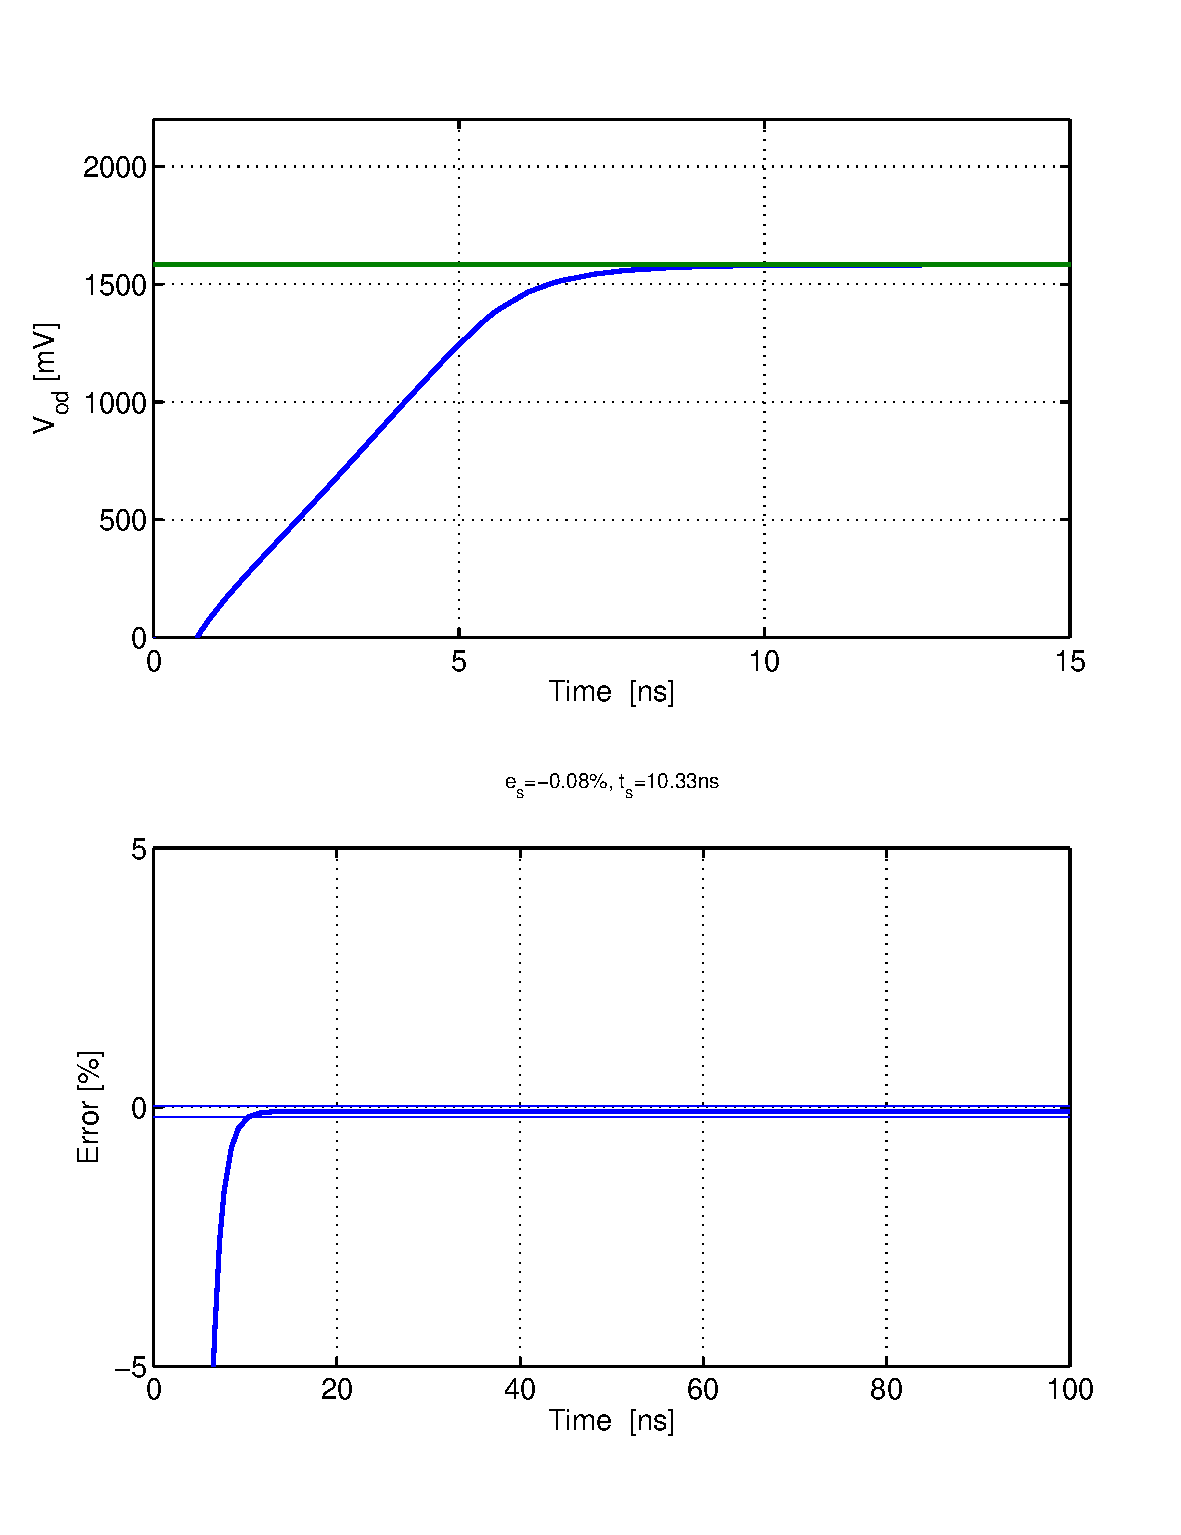
\includegraphics[width=0.8\textwidth]{common/ac.pdf}
    \end{center}
    \caption{AC仿真曲线}
    \label{commonac}
\end{figure}

% Page 6: Bode plot of T(j), phase and magnitude. Clearly annotate the achieved 
% low frequency loop gain, the loop crossover frequency and the phase margin.
\newpage
\clearpage
\subsection{输出范围}
直流仿真如图\ref{commondc},最大差模增益为$8045$,$70\%$的最大增益为$5631$,输出范围为$1.58\uV$。
\begin{figure}[htb]
    \begin{center}
        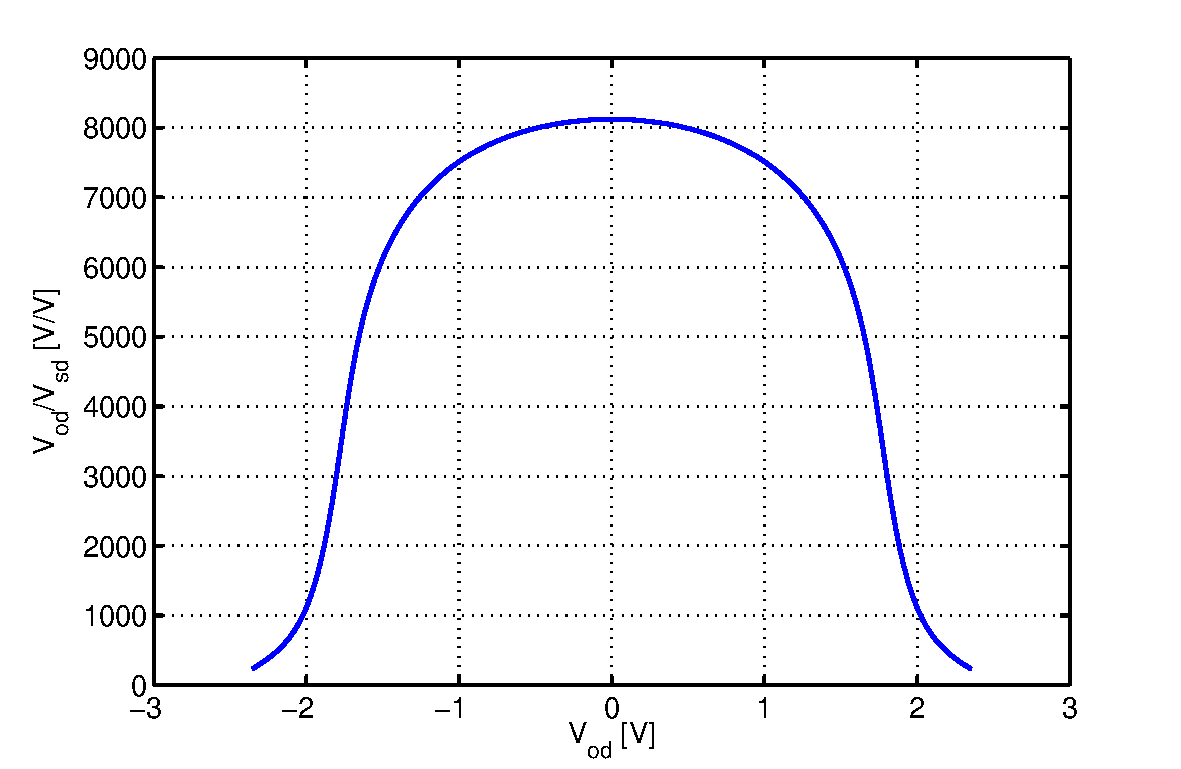
\includegraphics[width=0.8\textwidth]{common/dc.pdf}
    \end{center}
    \caption{DC仿真曲线}
    \label{commondc}
\end{figure}

\newpage
\clearpage
\subsection{噪声性能}

从图\ref{commonnoise}看到DR为$86.05\udB$,满足性能指标。
Telescopic 结构的缺点在于输出摆幅比较小,致使动态范围很难达到要求。
但也应注意到噪声小也是其主要优势,通过调节尽可能增大输出摆幅,
减小噪声可以提高动态范围。
\begin{figure}[htb]
    \begin{center}
        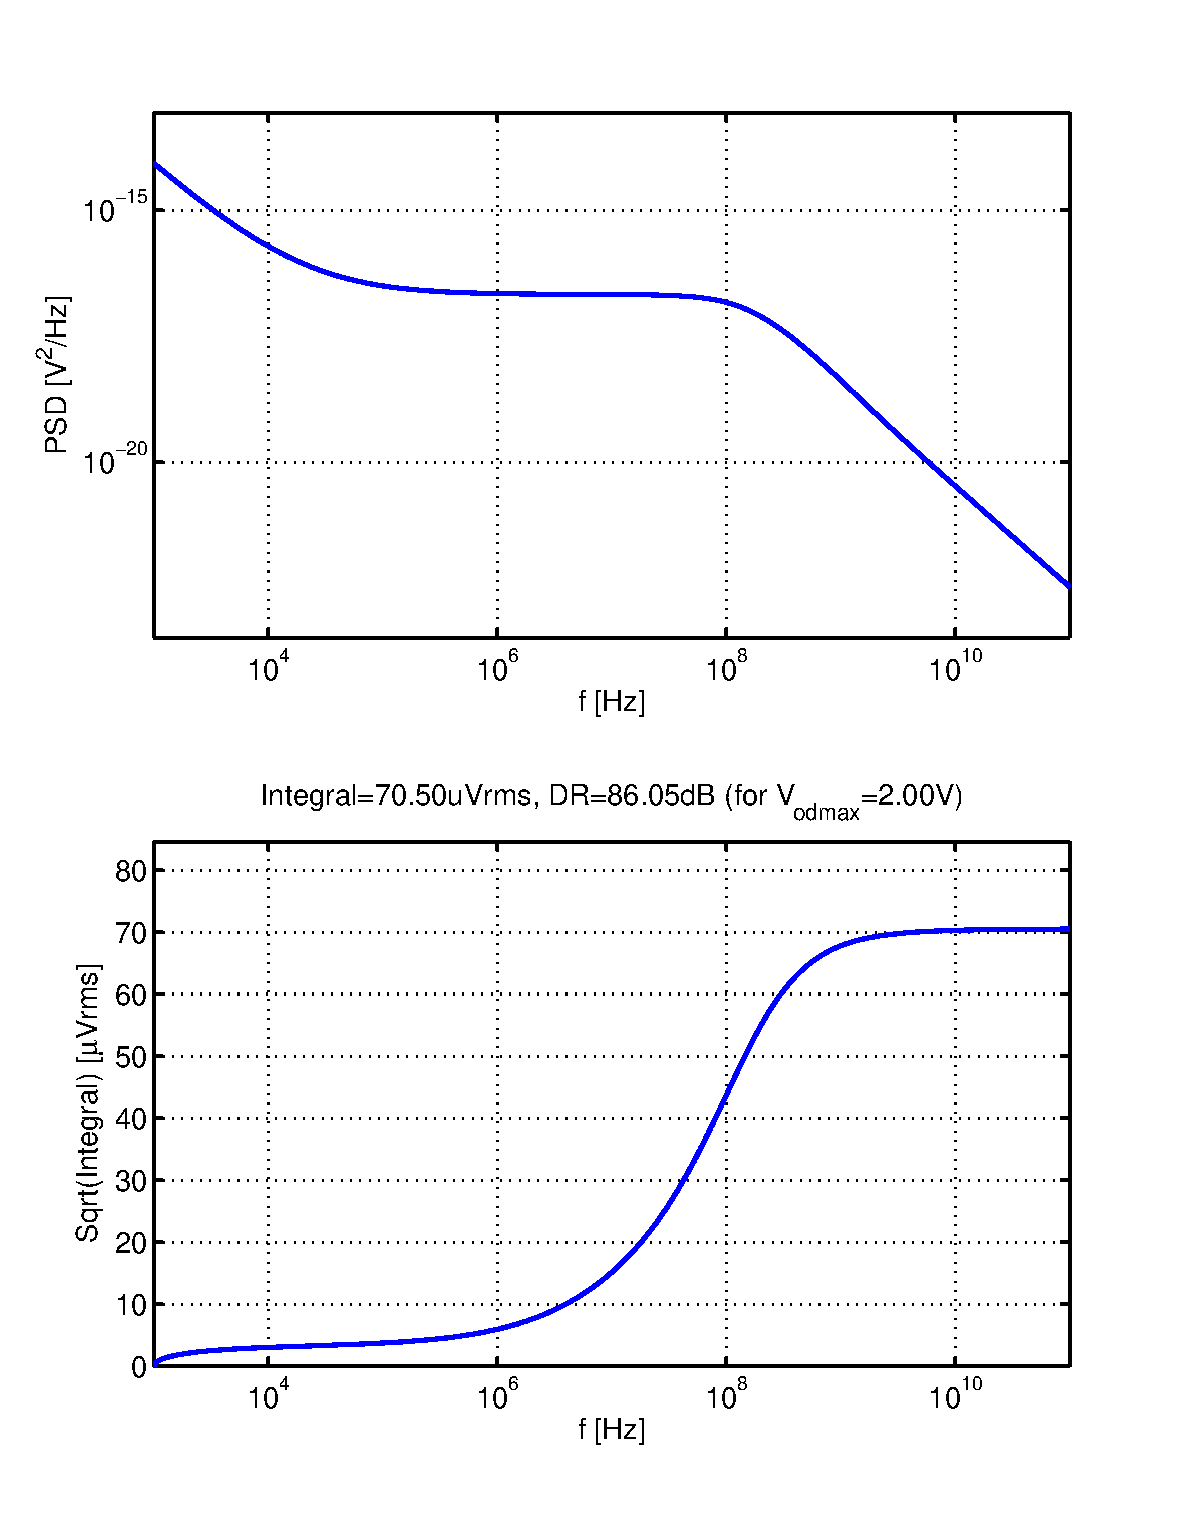
\includegraphics[width=0.8\textwidth]{common/noise.pdf}
    \end{center}
    \caption{噪声仿真曲线}
    \label{commonnoise}
\end{figure}

\newpage
\clearpage
\subsection{瞬态性能}
通过之前的DC仿真,已经知道输出摆幅。
设定参数为该值,在输出满摆幅的情况下,进行时序仿真,
静态误差为$0.08\%$。建立时间为$10.33\uns$,
满足要求。
\begin{figure}[htb]
    \begin{center}
        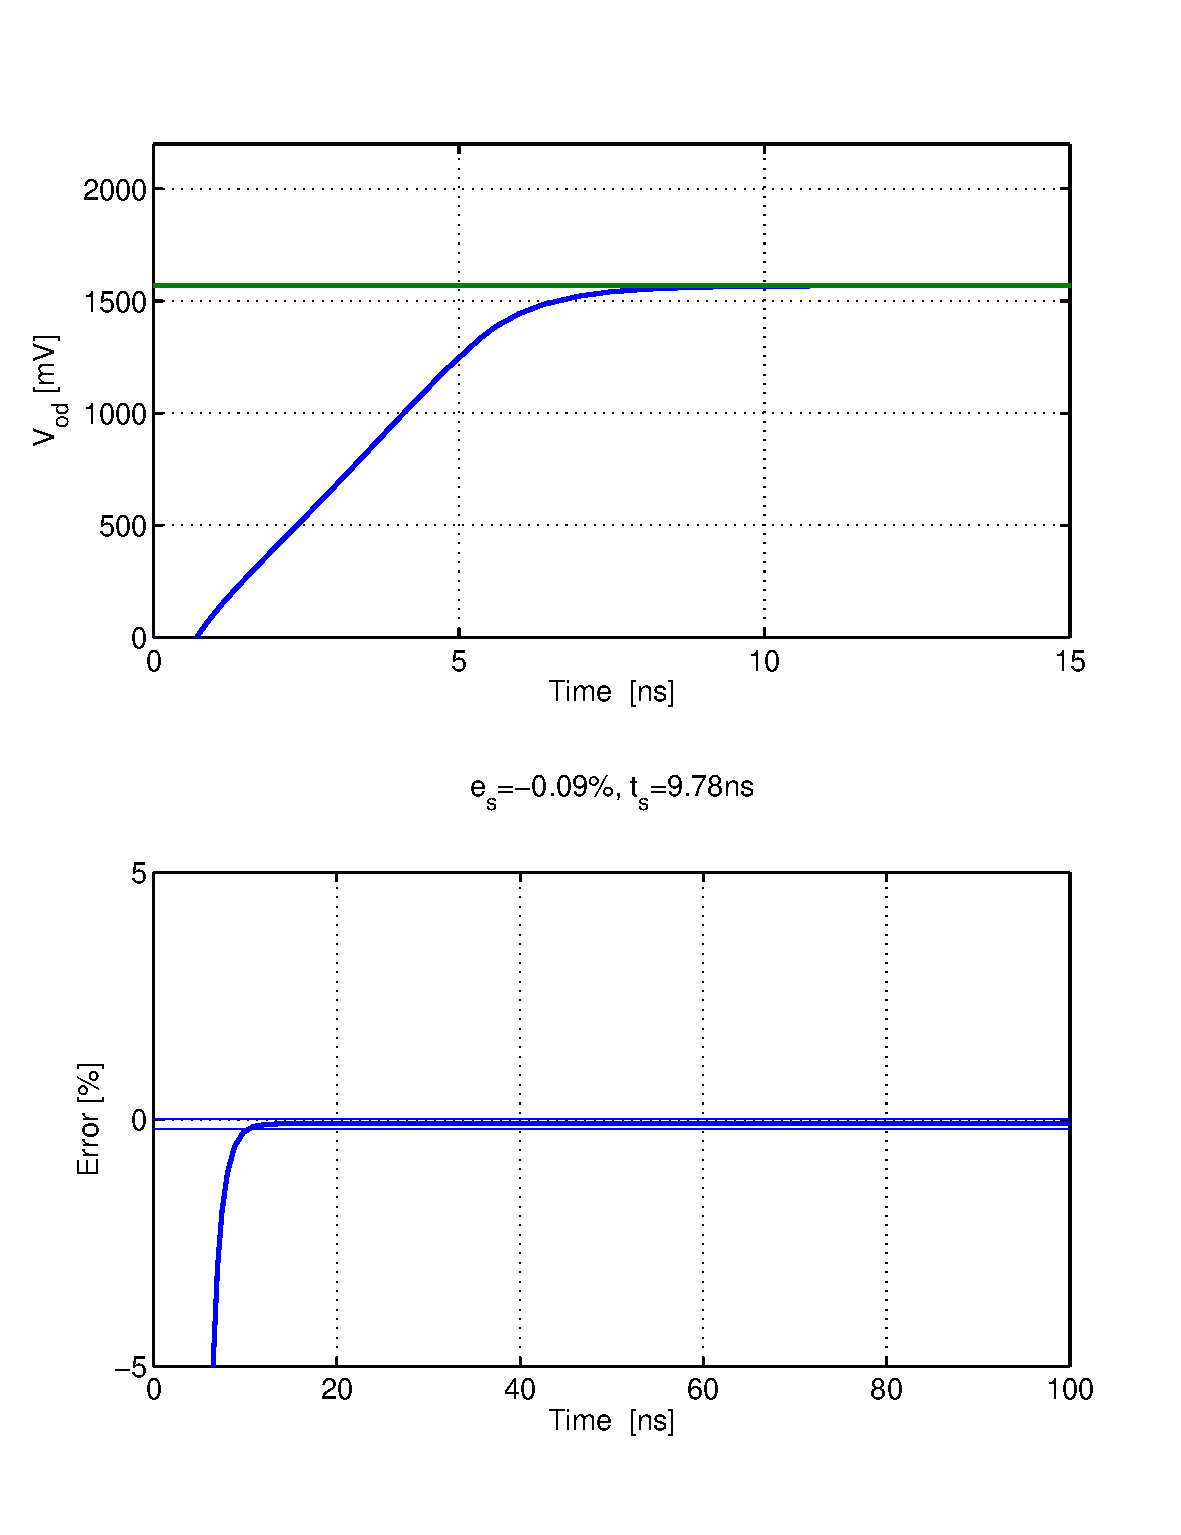
\includegraphics[width=0.8\textwidth]{common/tran1.pdf}
    \end{center}
    \caption{瞬态仿真曲线1}
    \label{commontran1}
\end{figure}

\begin{figure}[htb]
    \begin{center}
        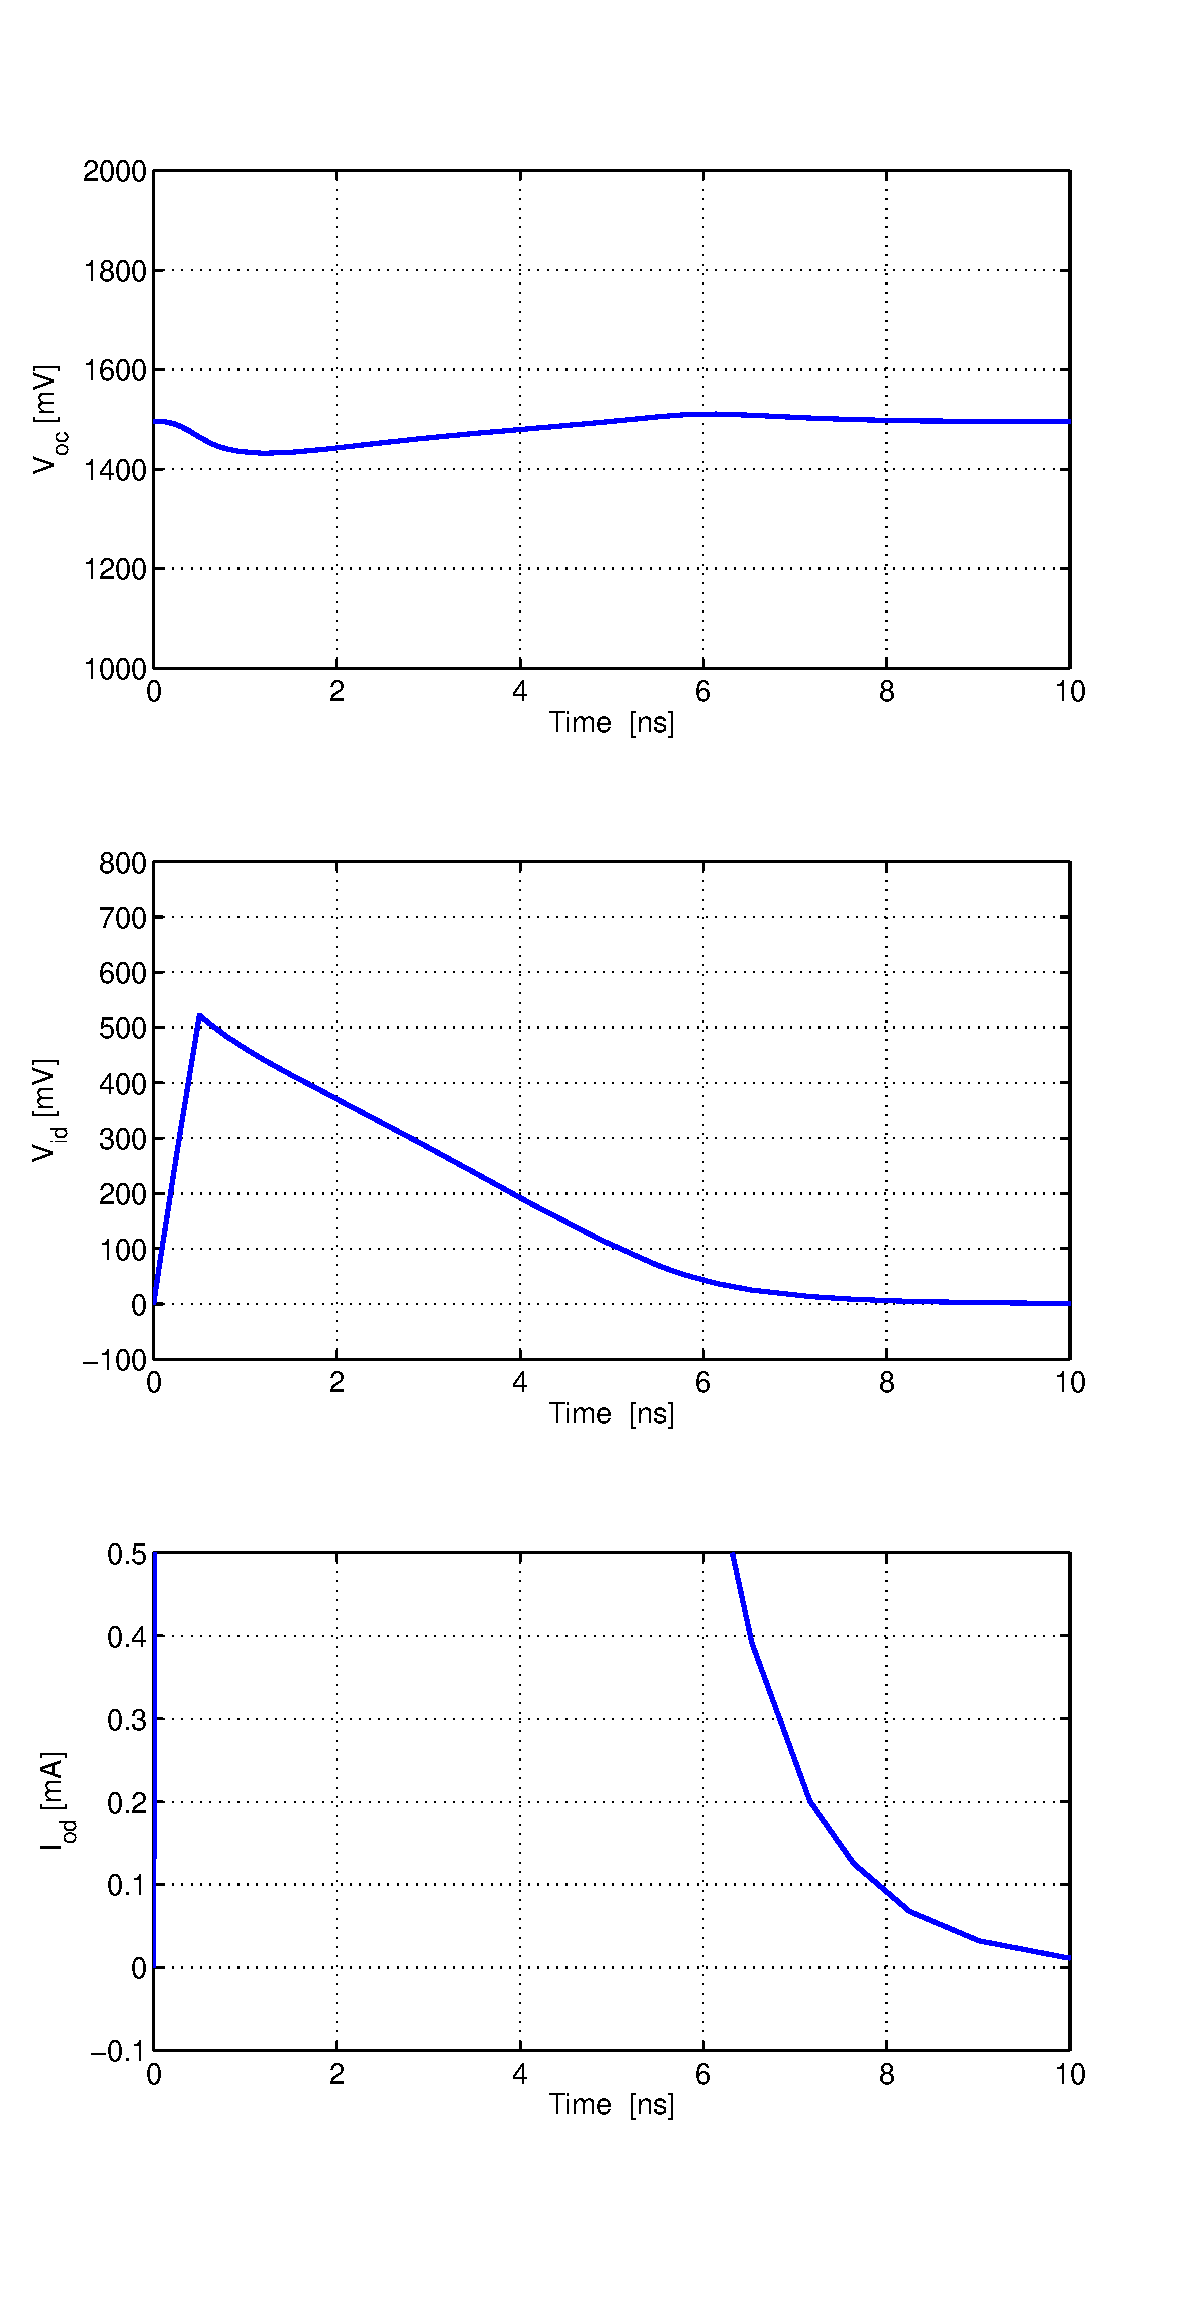
\includegraphics[width=0.8\textwidth]{common/tran2.pdf}
    \end{center}
    \caption{瞬态仿真曲线2}
    \label{commontran2}
\end{figure}
\newpage
\clearpage
\subsection{性能总结}
\begin{table}[htbp]
    \begin{tabular}{|c|c|}
        \hline
        dynamic range&$86.05\udB$
        \\\hline
        phase margin&$70.61\udeg$
        \\\hline
        $f_c$ &$107.42\uMHz$
        \\\hline 
        $T_0$&$1407$
        \\\hline
        $V_{odmax}$&$1.58\uV$
        \\\hline
        $t_s$($\varepsilon_s$=0.1\%)&$10.33\uns$
        \\\hline
        power consumption&$9.26\umW$
        \\\hline
        $C_l$&$2.3\upF$
        \\\hline
        $C_s$&$3.3\upF$
        \\\hline
    \end{tabular}
\end{table}

% Page 7: Plots the simulated settling transient of Vod (no zoom, show the 
% entire waveform). In a separate subplot, show the % error of the differential 
% output voltage relative to the ideal output voltage. Zoom into the relevant 
% region of the settling, i.e. clearly demonstrate that your
% design settles within spec. Annotate the achieved settling time and static 
% settling error. For simplicity, we use the error at t=30ns as an estimate of 
% the static settling error.  


% Page 8: Plot the common mode output voltage versus time during transient 
% settling of the circuit. In separate subplots each, also show the differential 
% output current of the OTA, and the differential input to the OTA (Vid in Figure 1).


% Page 9: Plot of the noise power spectral density at the OTA output (Vod) and 
% noise integral.  Annotate the total integrated noise value and the achieved 
% dynamic range.  

% Page 10: Output range. Simulation plot showing the differential open loop DC 
% gain Vod/Vid of the amplifier. Mark the differential output voltage at which 
% the gain has dropped by 30%.  This value should be larger than the peak output 
% voltage used in your dynamic range calculation.

% Page 11-12: Results of corner simulations. Tabulate your circuit’s performance 
% for the slow/hot and fast/cold corner. Include settling time, static error, 
% and any other parameter that you find noteworthy. Include the %-changes with 
% respect to nominal conditions in your table.
% In case the circuit is non-functional in these corners, investigate and explain 
% the problem (no need to fix the circuit). Include selected interesting plots 
% documenting corner performance and/or issues.

\clearpage
\newpage

\section{slow corner路性能}
\subsection{AC仿真频率特性}
\begin{figure}[htb]
    \begin{center}
        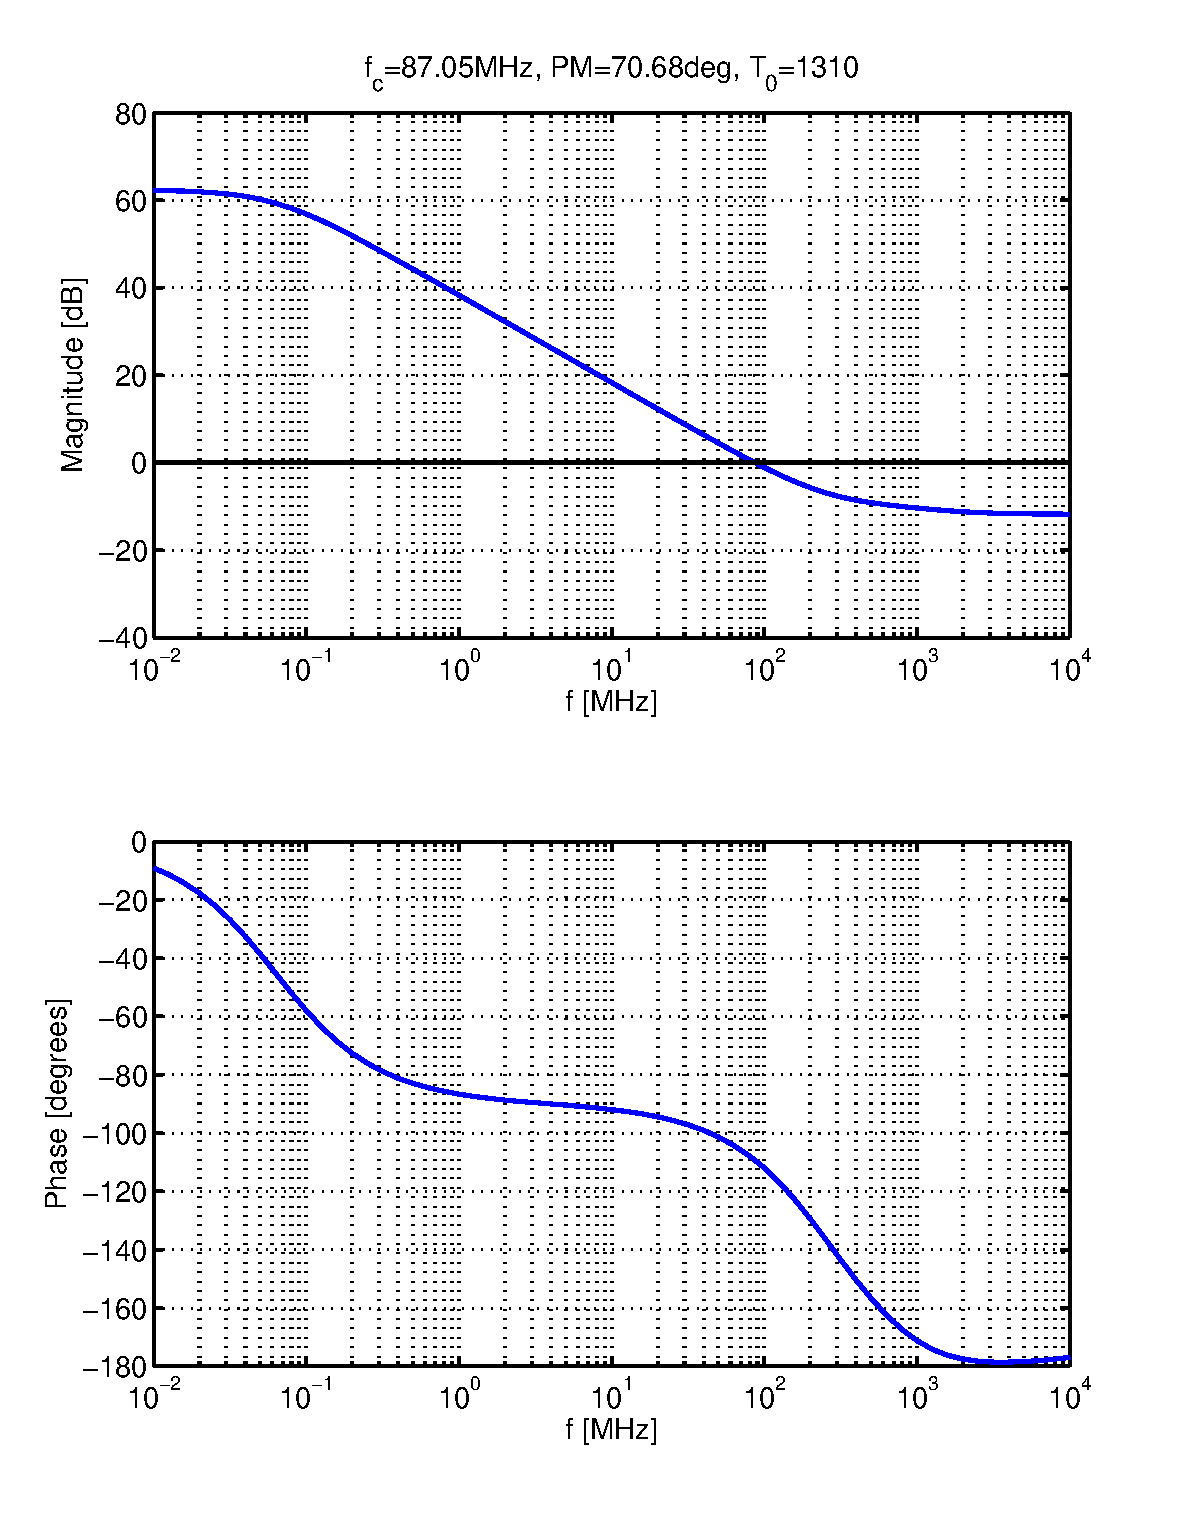
\includegraphics[width=\textwidth]{slow/ac.pdf}
    \end{center}
    \caption{AC仿真曲线}
    \label{slowac}
\end{figure}
电路幅频曲线,相频曲线如图\ref{slowac}所示。
可以看到低频闭环增益为$1319$,相位裕度为$70.66\udeg$,闭环跨导频率$1319$。
% Page 6: Bode plot of T(j), phase and magnitude. Clearly annotate the achieved 
% low frequency loop gain, the loop crossover frequency and the phase margin.
\newpage
\clearpage
\subsection{输出范围}
\begin{figure}[htb]
    \begin{center}
        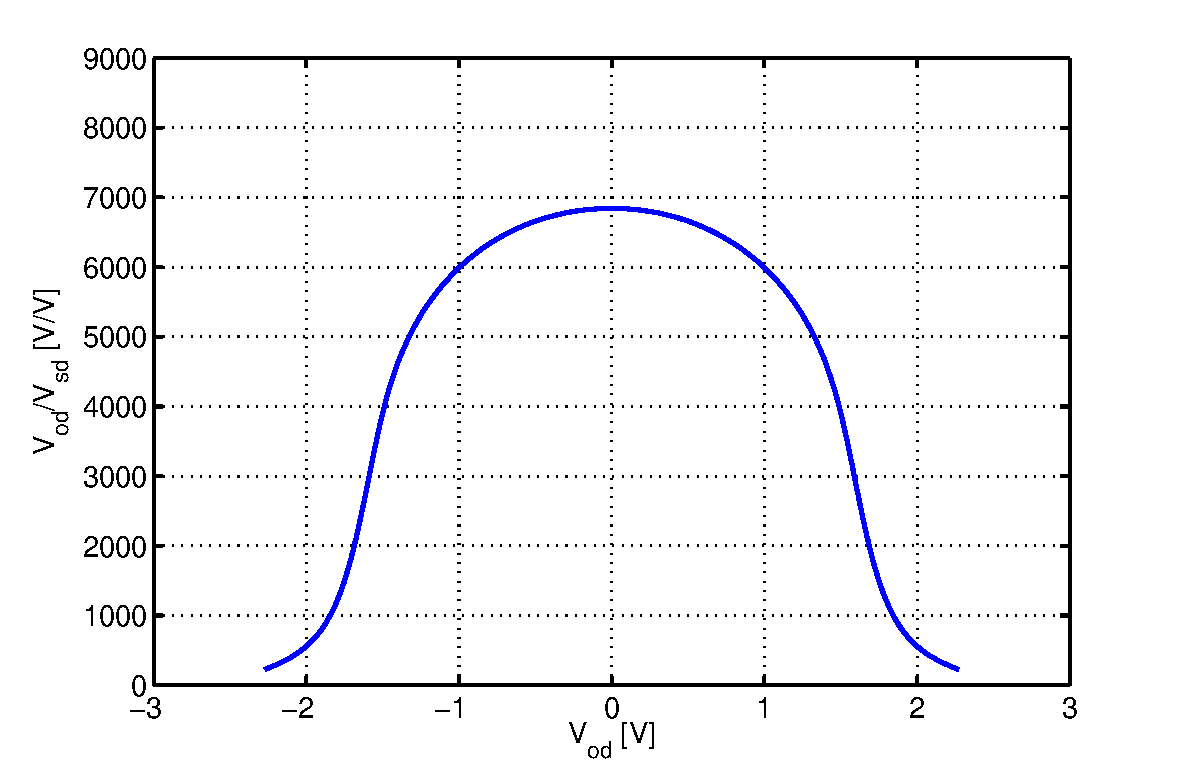
\includegraphics[width=\textwidth]{slow/dc.pdf}
    \end{center}
    \caption{DC仿真曲线}
    \label{slowdc}
\end{figure}
输出范围为$1.39\uV$。输出摆幅比原数据略小。
\newpage
\clearpage
\subsection{噪声性能}
\begin{figure}[htb]
    \begin{center}
        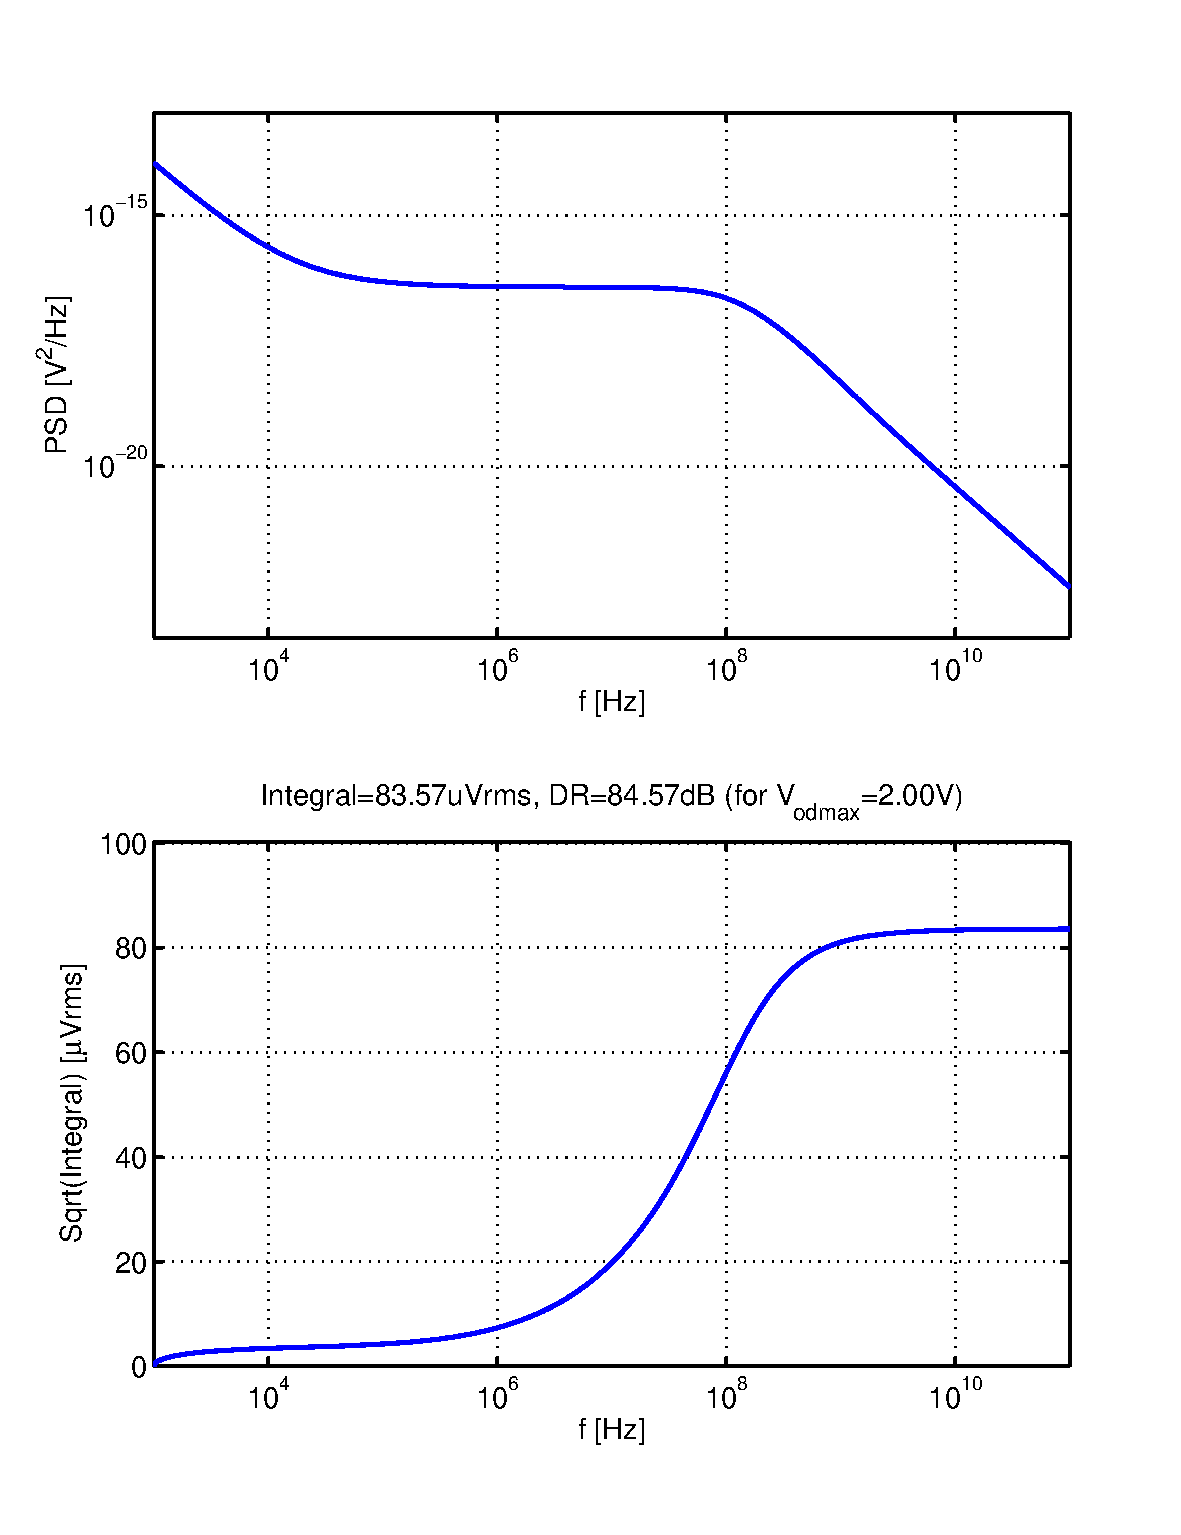
\includegraphics[width=\textwidth]{slow/noise.pdf}
    \end{center}
    \caption{noise仿真曲线}
    \label{slownoise}
\end{figure}
从图中看到DR为$84.57\udB$。噪声特性DR变小。
\newpage
\clearpage
\subsection{瞬态性能}

\begin{figure}[htb]
    \begin{center}
        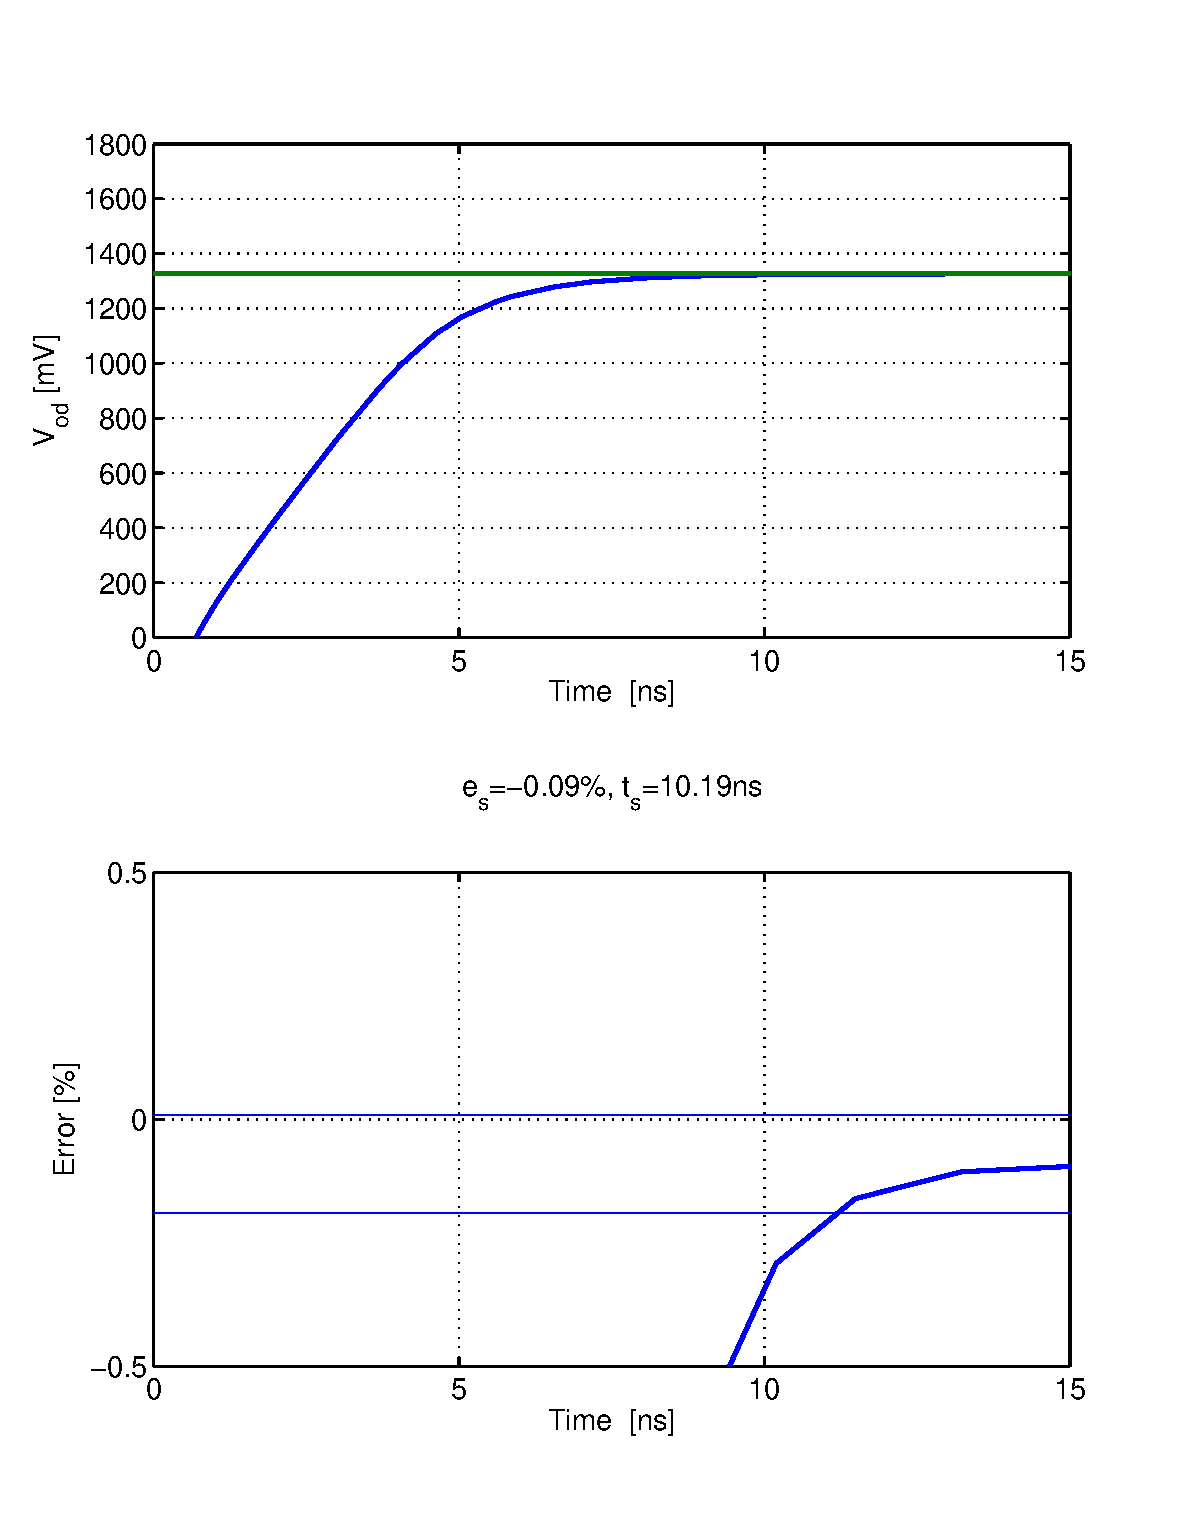
\includegraphics[width=\textwidth]{slow/tran1.pdf}
    \end{center}
    \caption{noise仿真曲线1}
    \label{slowtran1}
\end{figure}

\begin{figure}[htb]
    \begin{center}
        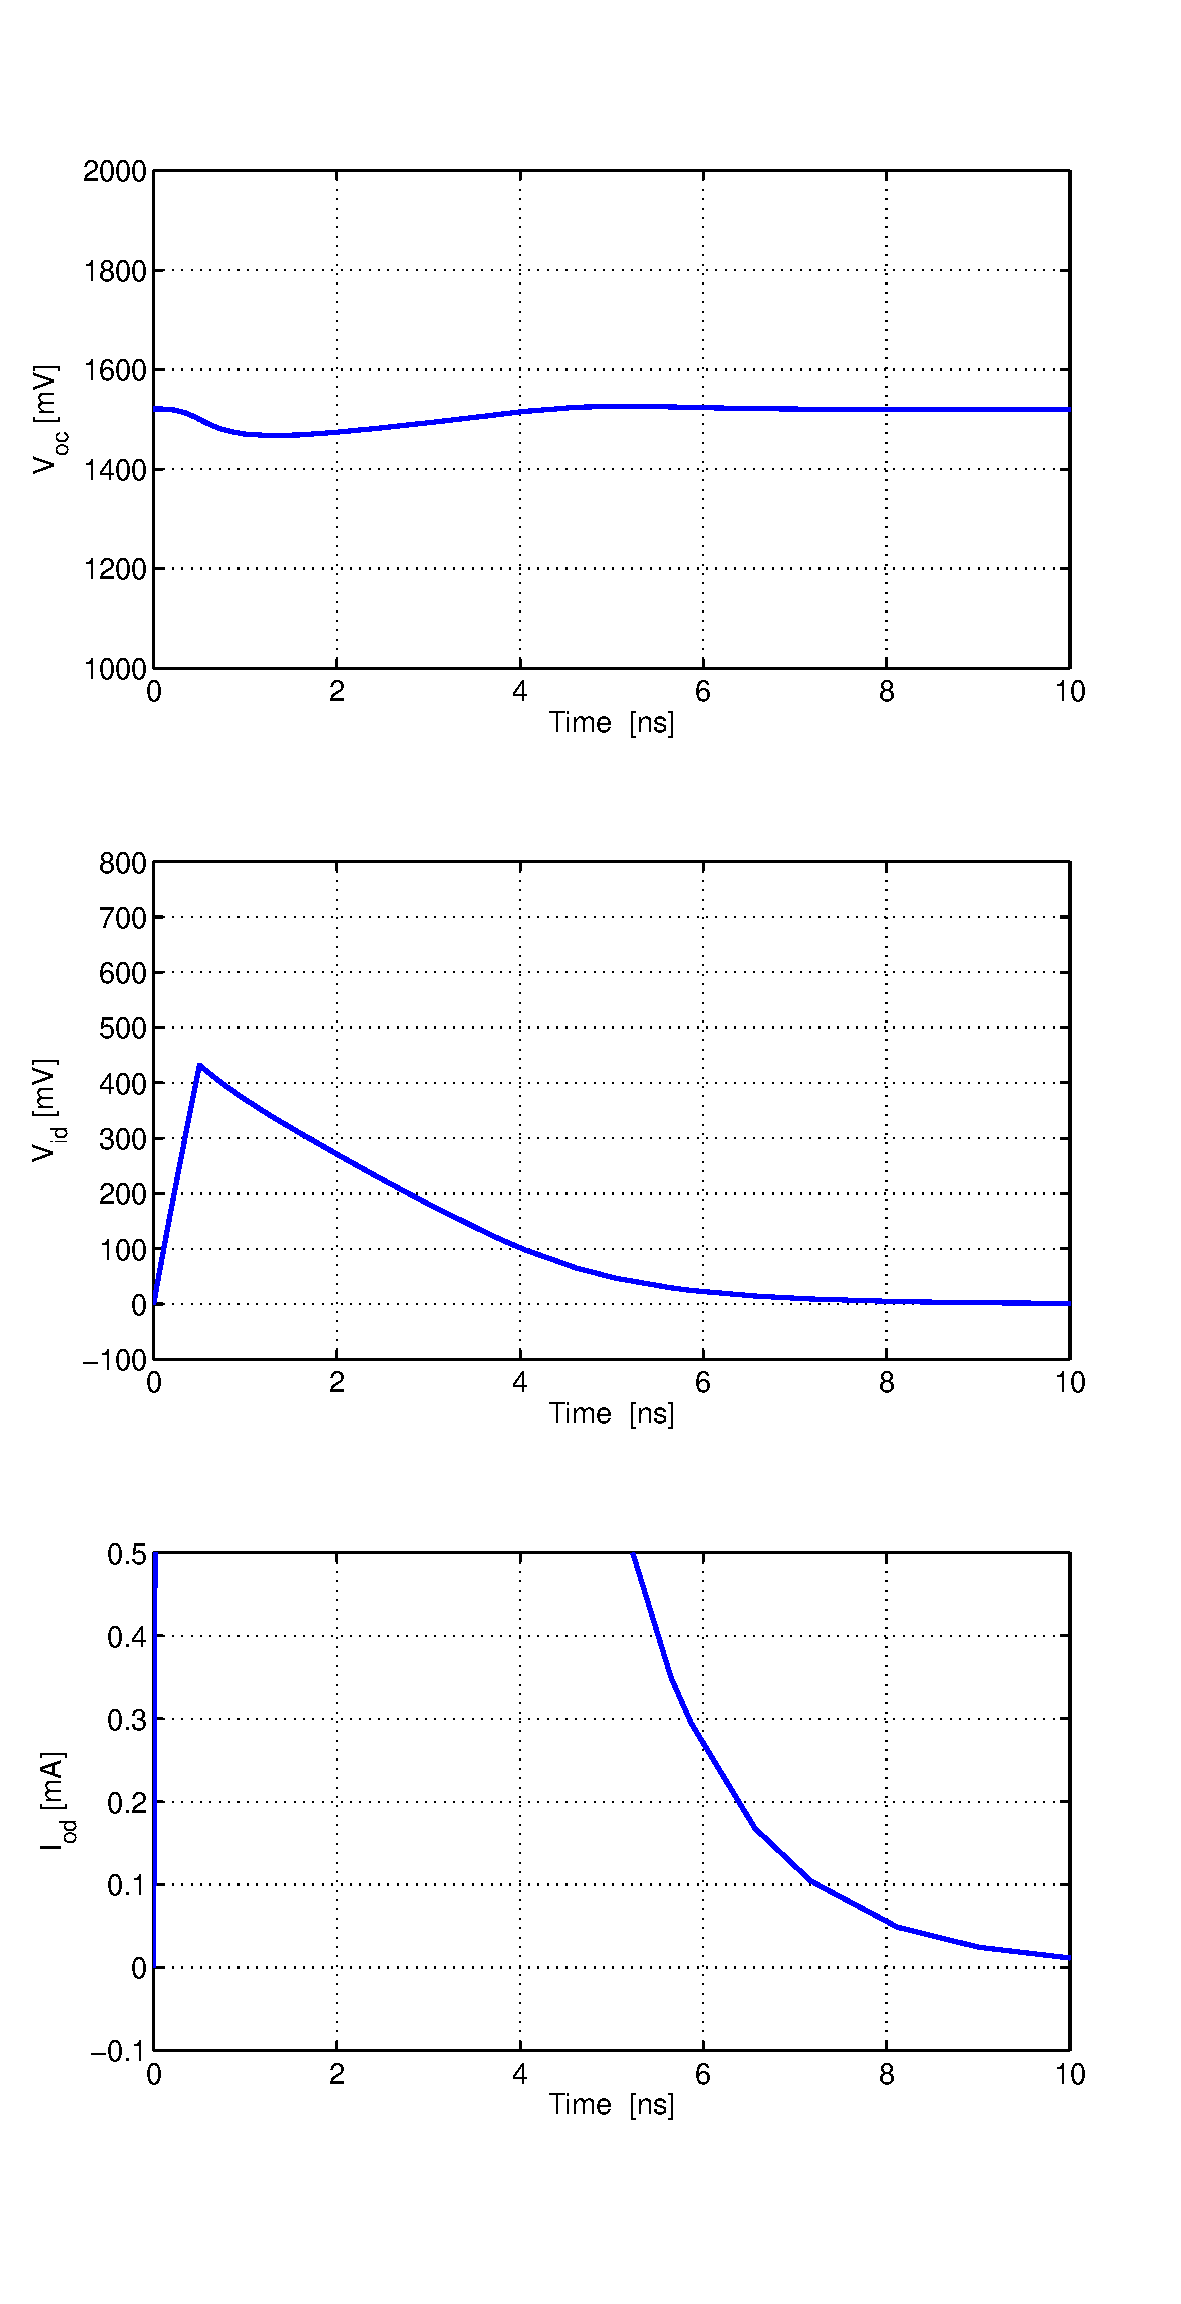
\includegraphics[width=\textwidth]{slow/tran2.pdf}
    \end{center}
    \caption{noise仿真曲线2}
    \label{slowtran2}
\end{figure}
可以看出静态误差变大,线性建立时间变大。

\newpage
\clearpage
\subsection{性能总结}

\begin{table}[htbp]
    \begin{tabular}{|c|c|}
        \hline
        dynamic range&$84.57\udB$
        \hline
        phase margin&$70.66\udeg$
        \hline
        $f_c$ &$86.65\uMhHZ$
        \hline 
        $T_0$&$1319$
        \hline
        $V_{odmax}$&$1.37\uV$
        \hline
        $t_s$($\varepsilon_s$=0.1\%)&$11.89\uns$
        \hline
        power consumption&$9.42\umW$
        \hline
        $C_l$&$2.3\upF$
        \hline
        $C_s$&$3.3\upF$
        \hline
    \end{tabular}
\end{table}
\newpage
\clearpage

\section{fast corner路性能}
\subsection{AC仿真频率特性}
\begin{figure}[htb]
    \begin{center}
        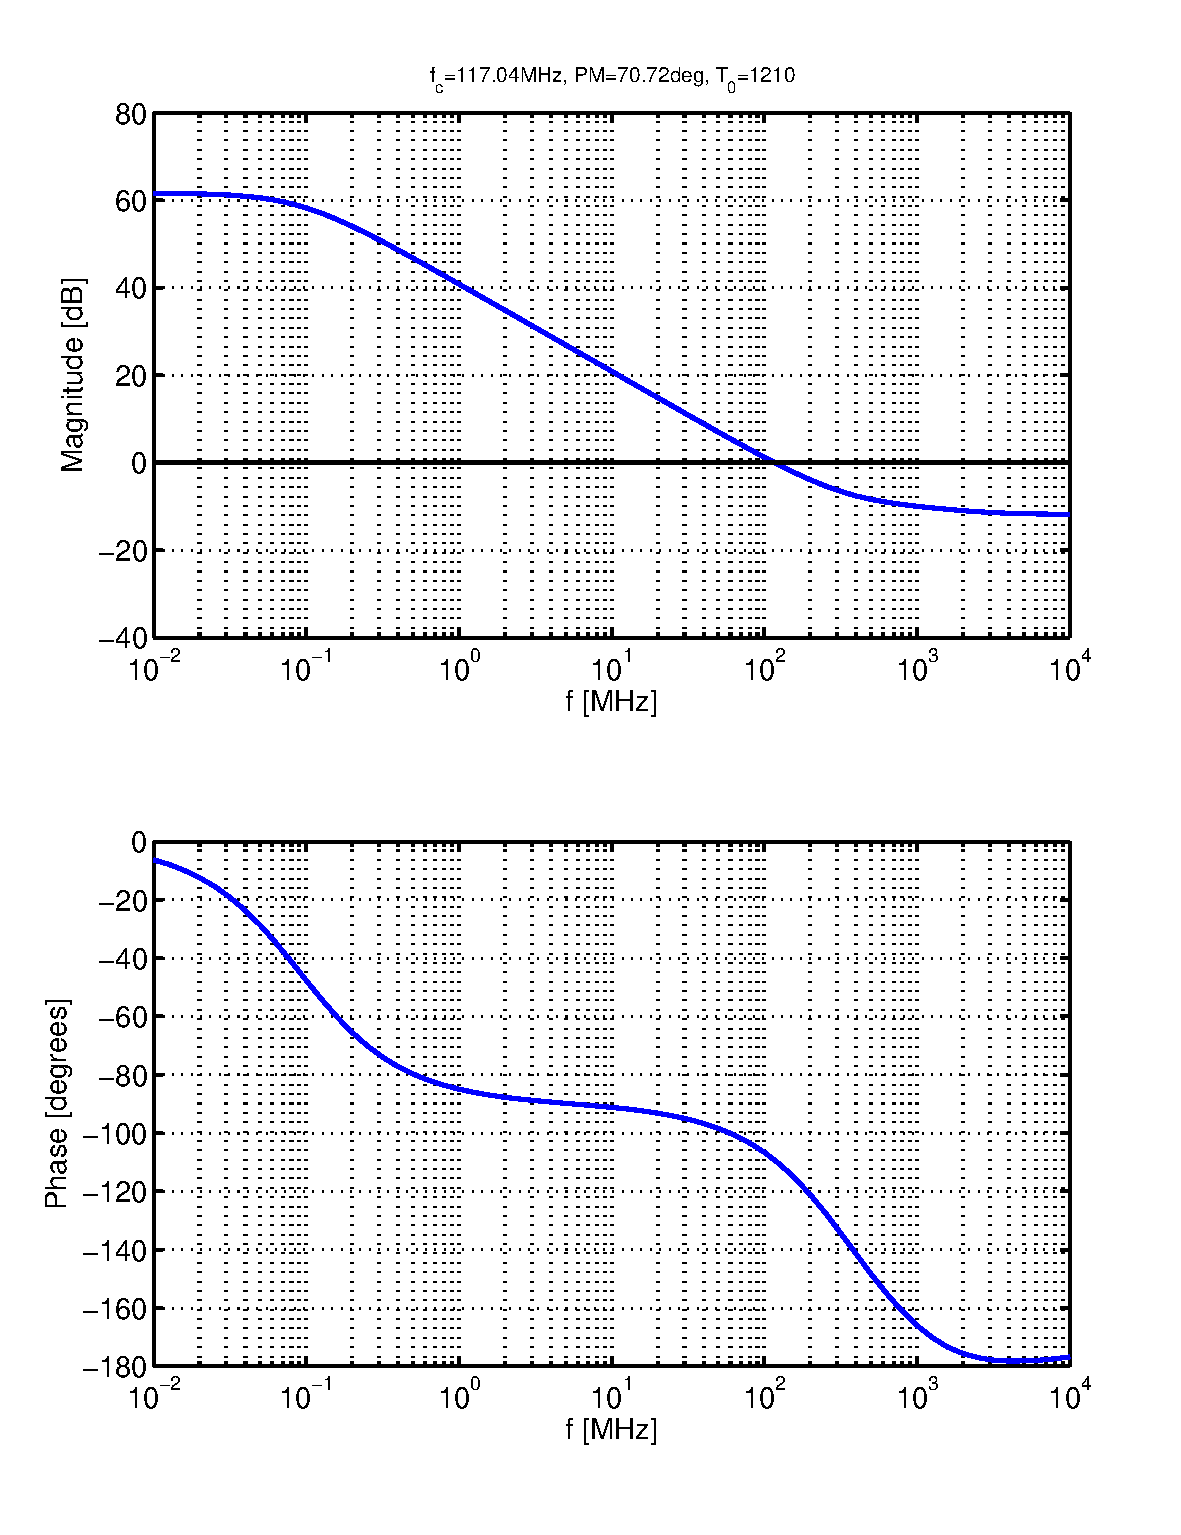
\includegraphics[width=\textwidth]{fast/ac.pdf}
    \end{center}
    \caption{AC仿真曲线}
    \label{fastac}
\end{figure}
电路幅频曲线,相频曲线如图\ref{fastac}所示。
可以看到低频闭环增益为$1210$,相位裕度为$70.72\udeg$,闭环跨导频率$1210$。
可以发现负反馈增益和带宽有相互抑制的关系。
% Page 6: Bode plot of T(j), phase and magnitude. Clearly annotate the achieved 
% low frequency loop gain, the loop crossover frequency and the phase margin.
\newpage
\clearpage
\subsection{输出范围}
\begin{figure}[htb]
    \begin{center}
        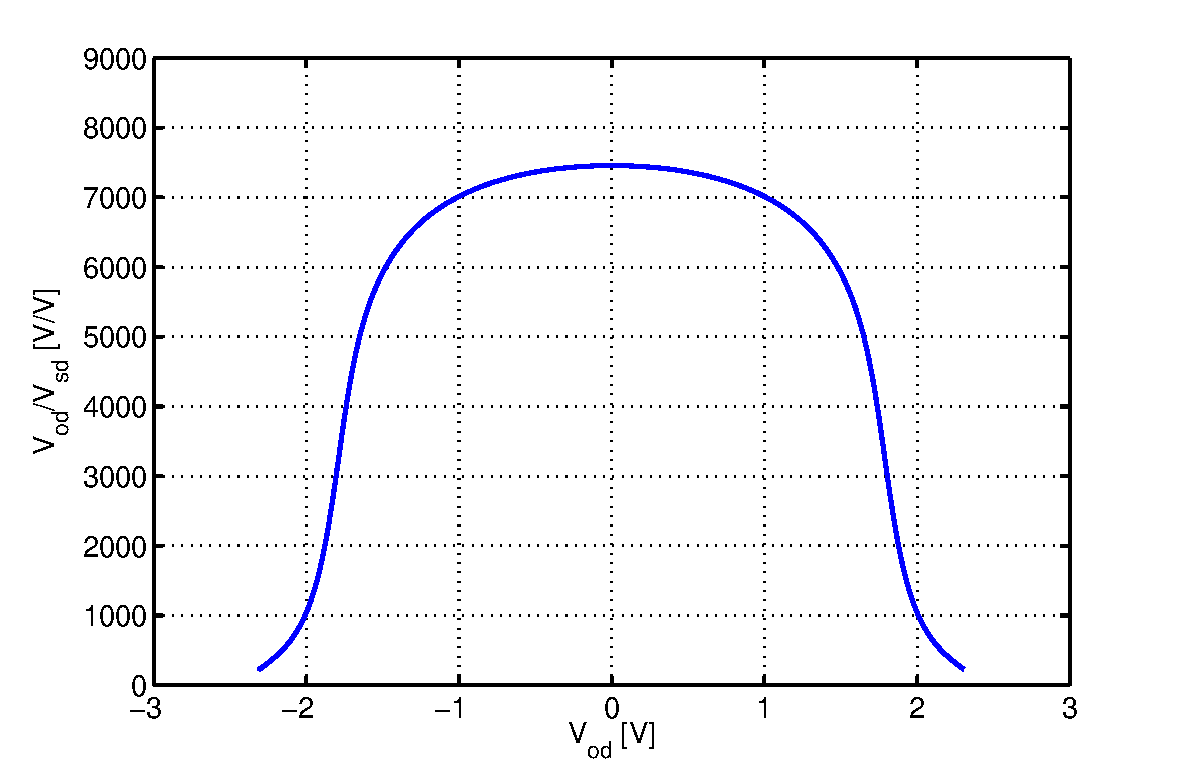
\includegraphics[width=\textwidth]{fast/dc.pdf}
    \end{center}
    \caption{DC仿真曲线}
    \label{fastdc}
\end{figure}
%\ref{dc}
输出范围为$1.61\uV$。输出摆幅比原数据略大。
\newpage
\clearpage
\subsection{噪声性能}
\begin{figure}[htb]
    \begin{center}
        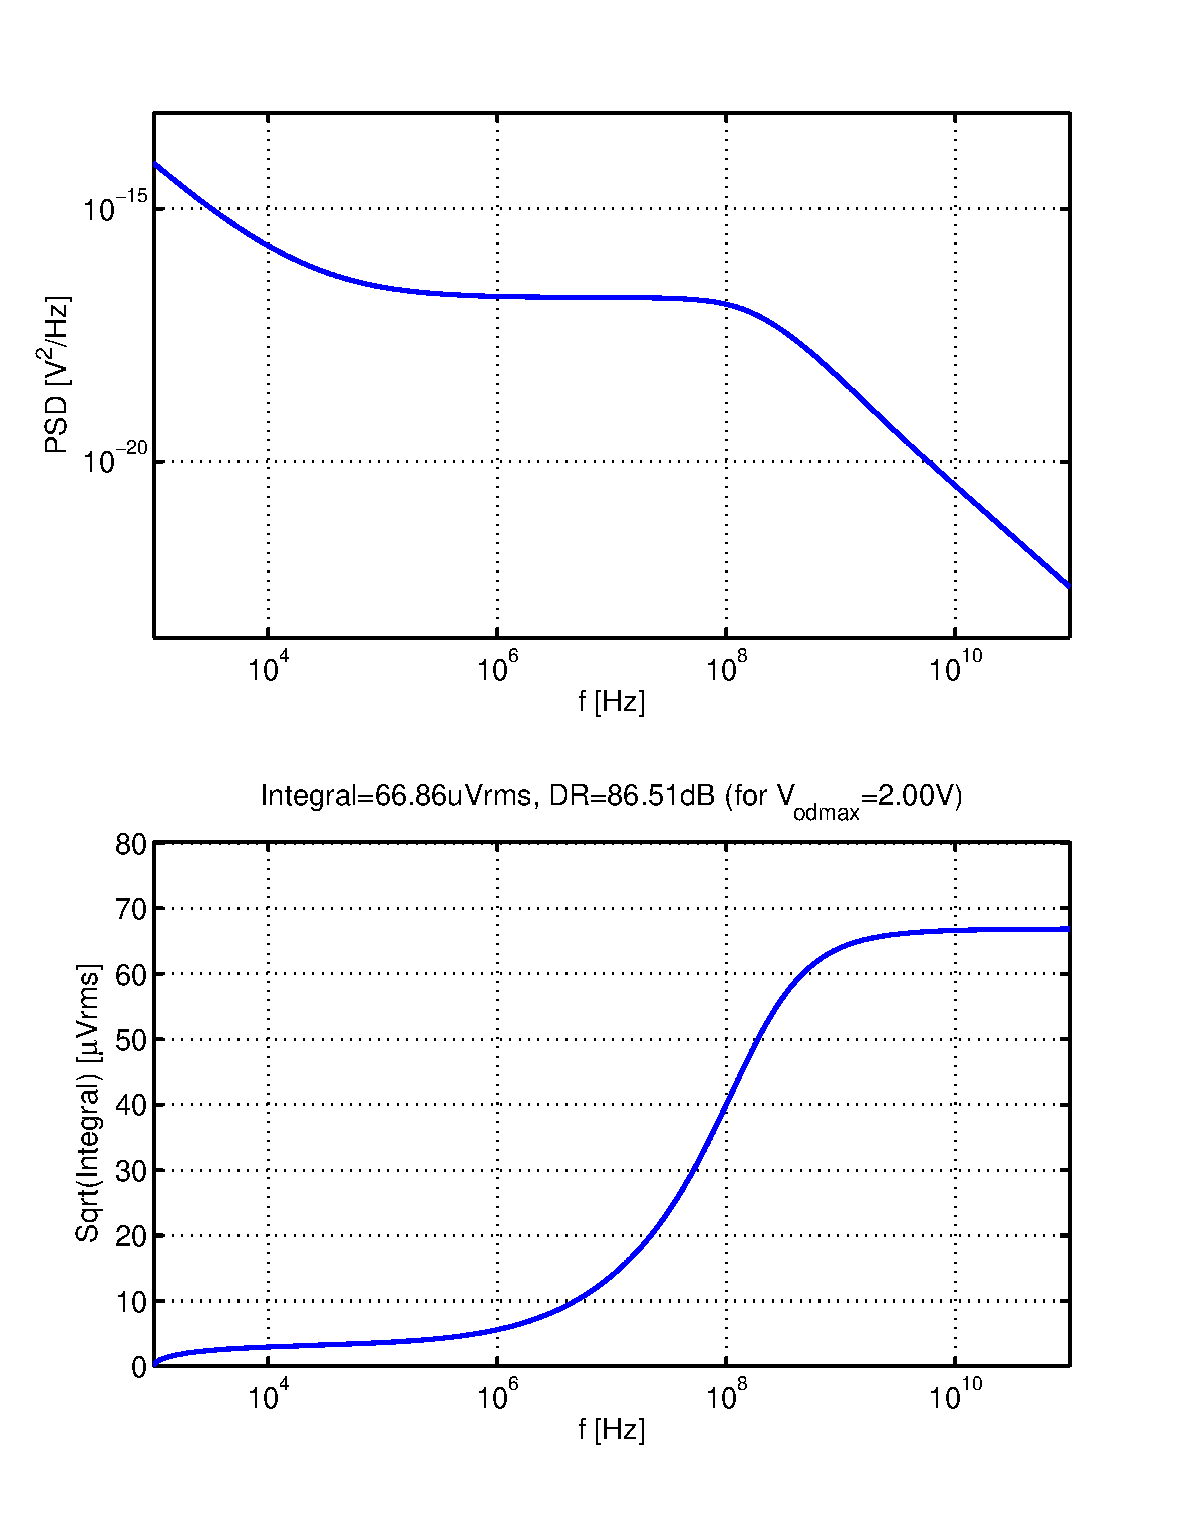
\includegraphics[width=\textwidth]{fast/noise.pdf}
    \end{center}
    \caption{noise仿真曲线}
    \label{fastnoise}
\end{figure}
从图中看到DR为$86.52\udB$。噪声特性DR变大。
\newpage
\clearpage
\subsection{瞬态性能}

\begin{figure}[htb]
    \begin{center}
        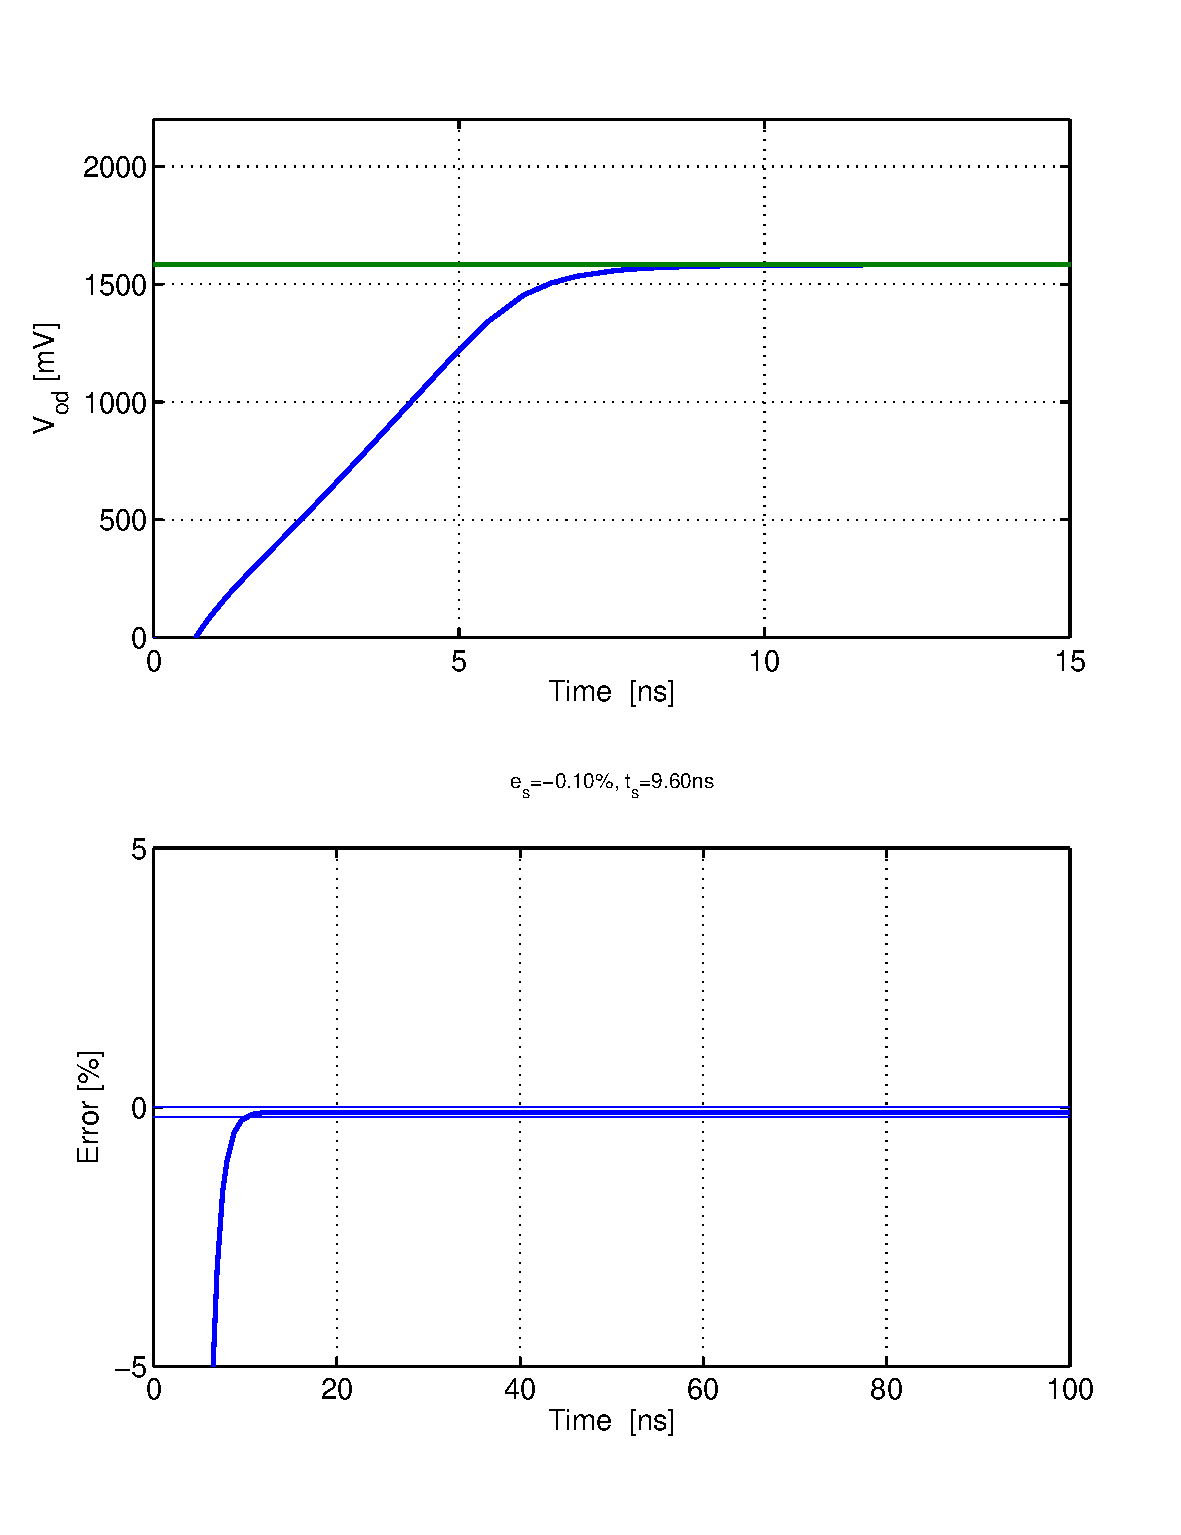
\includegraphics[width=\textwidth]{fast/tran1.pdf}
    \end{center}
    \caption{noise仿真曲线1}
    \label{fasttran1}
\end{figure}

\begin{figure}[htb]
    \begin{center}
        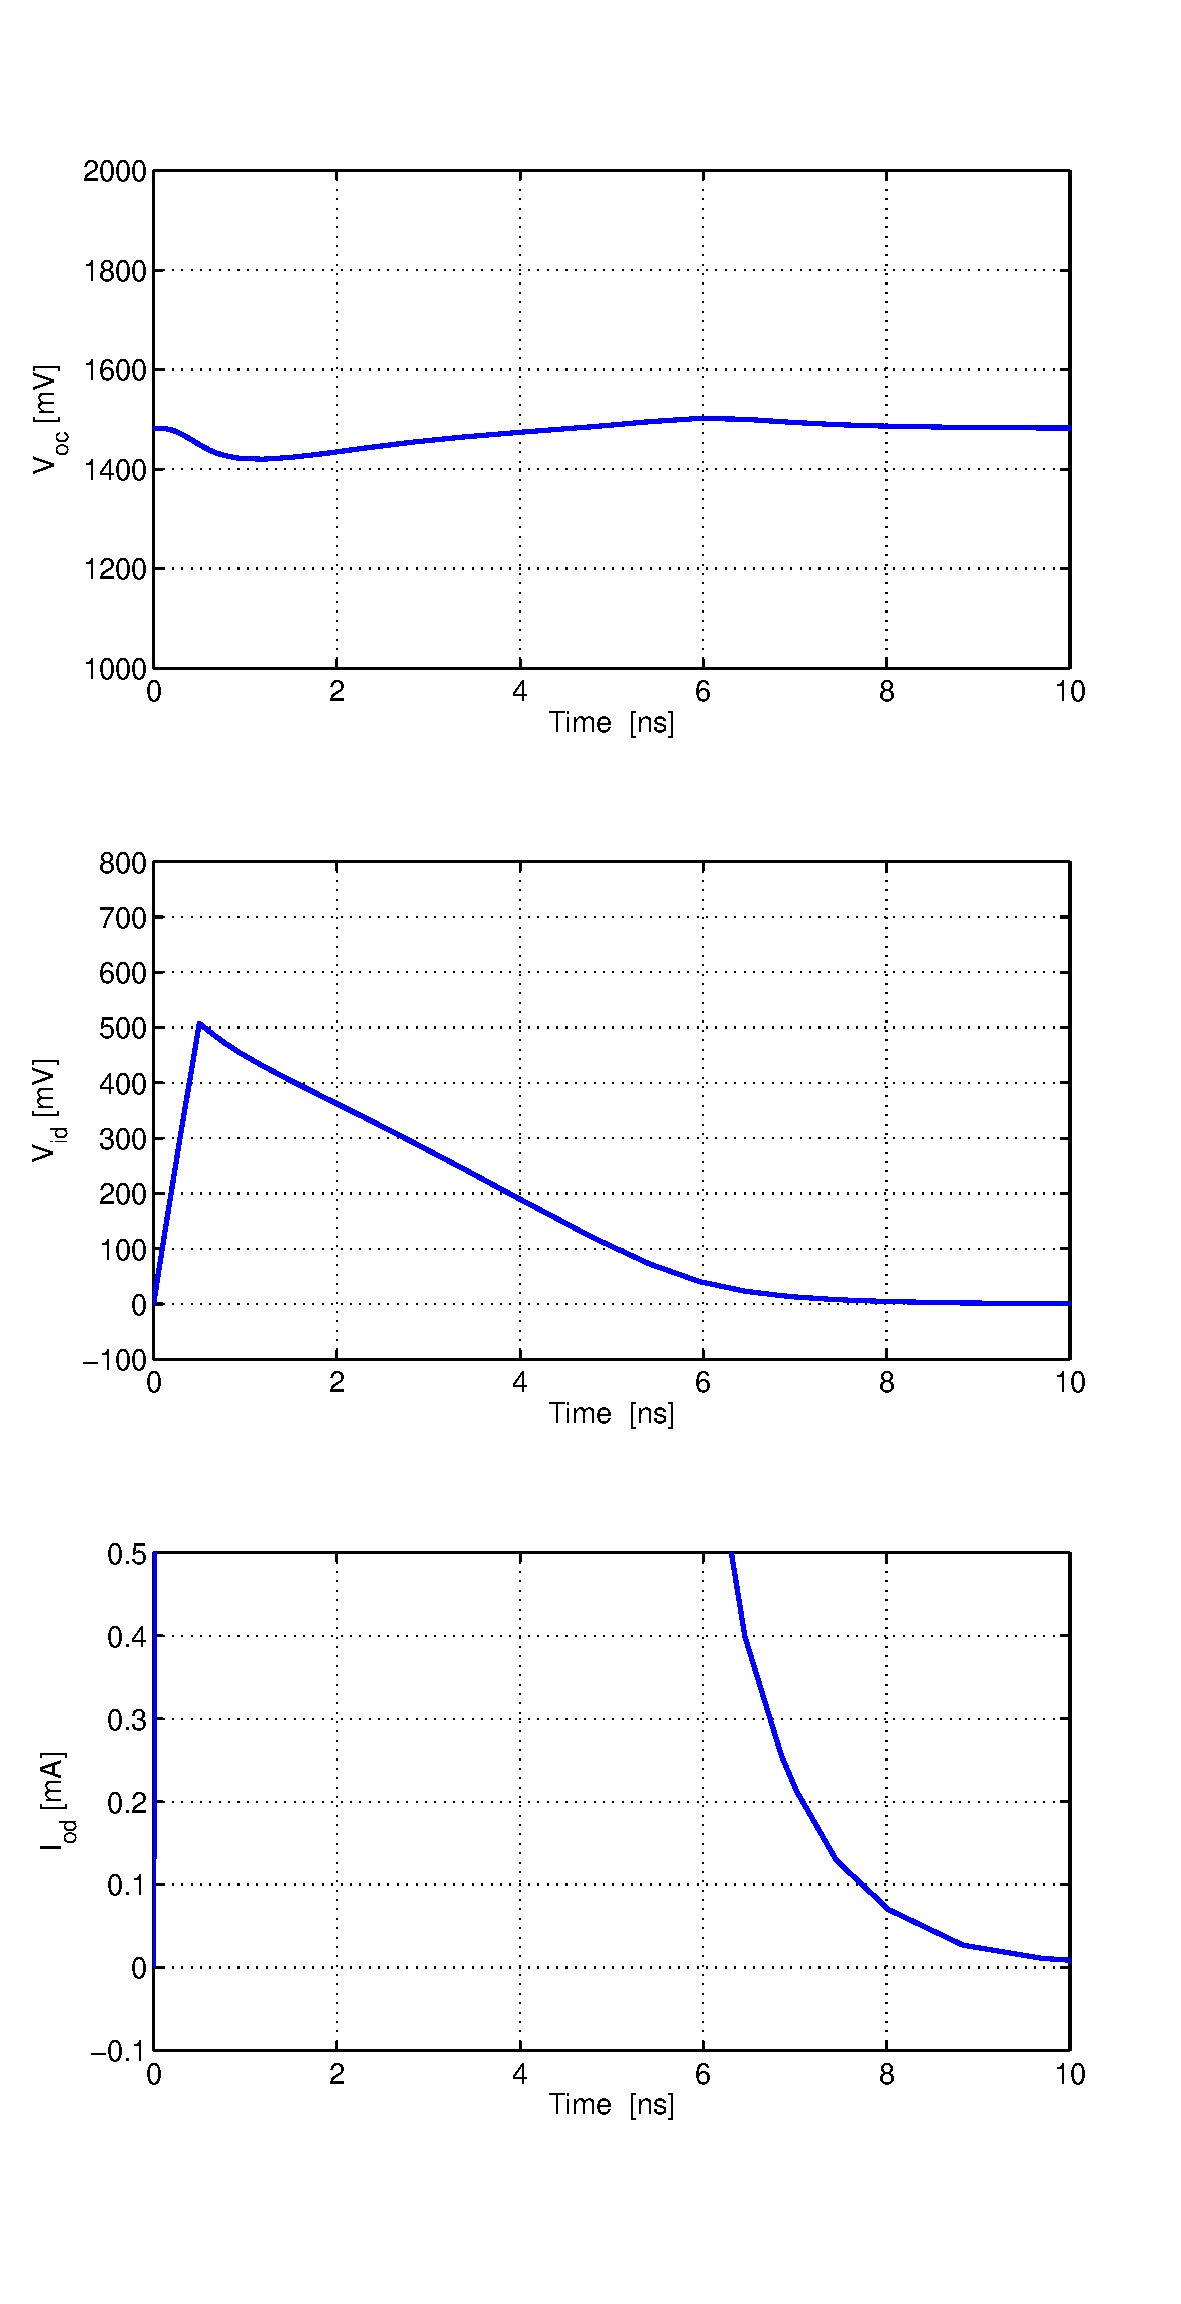
\includegraphics[width=\textwidth]{fast/tran2.pdf}
    \end{center}
    \caption{noise仿真曲线2}
    \label{fasttran2}
\end{figure}
可以看出静态误差变大,线性建立时间变小。

\newpage
\clearpage
\subsection{性能总结}

\begin{table}[htbp]
    \begin{tabular}{|c|c|}
        \hline
        dynamic range&$86.52\udB$
        \hline
        phase margin&$70.72\udeg$
        \hline
        $f_c$ &$117.04\uMhHZ$
        \hline 
        $T_0$&$1210$
        \hline
        $V_{odmax}$&$1.61\uV$
        \hline
        $t_s$($\varepsilon_s$=0.1\%)&$9.6\uns$
        \hline
        power consumption&$9.29\umW$
        \hline
        $C_l$&$2.3\upF$
        \hline
        $C_s$&$3.3\upF$
        \hline
    \end{tabular}
\end{table}


% Page 13: Comments and Conclusion. Here, you can convey issues you may have had, 
% or things you’ve learned/not learned in this project.
\section{结论与总结}
本次project使我对OTA设计有了更深的理解。书本上轻描淡写几笔带过的设计流程,
在实际设计中却有着复杂而错综复杂的关联关系。从前期对电路结构的选择,到最终
选择Telescopic结构,对于不同OTA的特点有了更深的理解。集成了手工计算,
matlab仿真,以及后期调整迭代的project,使我们对于设计流程有了更
深入的体会。并且对各个参数指标之间的关系进行了思考和分析,整理了这些互相交织的概念
。通过对课本基本两级 OTA 的设计案例的分析,参照其流程和思路,我们
经过多次修改和调试完成了本次课程设计。在调试和修改的过程中,我感触最深刻的
是电路性能之间的互相关联以及为达到设计指标所做出的折衷。为了换得到较小的动态误差,
我们相应牺牲了一些相位裕量和并加大了一些功耗。
这样的妥协还有很多,正是在权衡考虑之间,才能更好的设计出满足设计指标的电路。

另外,课程设计中涉及到的电路复杂,结构互相关联。project要求中模块化设计的设计思路,
对于我们很有帮助。各个电路结构成一个个子系统
,电路参数提取时分成一个个小文件,这样可以防止我们在纷多的设计参数中迷乱,
在复杂的电路前束手无策。在分析偏置模块和差分负反馈模块的性能,明确各个管子在电路中的作用,仿真
过程中更有针对性地对关键晶体管反复进行参数修改过程中,模块化设计保证了调试的有效进行。

最后,值得一提的是在本次设计中大量使用了自动化脚本进行数据分析。因为脚本的大量使用,我们可以实现在
命令行中输入一个命令,就可以将调整过设计要求的电路参数自动输出到文件,之后再include进入hspice仿真
完整之后的工作,再一次性完成多个技术参数的提取。通过这样的步骤,大大简化了较为繁琐的手续,可以更加高效的完成
后面的设计。

课程设计汇报时助教候老师提出的建议对我们后续的修改和优化起到了较大的帮助,在这里感谢助教老师。
在整个报告的最后,将感谢献给小组的成员。日日夜夜的奋斗得到的不仅仅是一个project,
更是对于问题的思考,对于困难的无畏,对于更高标准的坚持,对于合作的推崇。很多问题自己琢磨很久没有头绪,
在和大家一起讨论分析之后问题能够逐渐被解决。相信所有的这一切都会成为大家共同的回忆。



\end{document}

